\renewcommand{\nomducours}{\nomcoursneuf}
\renewcommand{\chapterlabel}{chap_neuf}
\renewcommand{\sousnomducours}{\sousnomcoursneuf}
\renewcommand{\contentsummaryducours}{\contentsummarycoursneuf}

\chapter{\nomducours}
\thispagestyle{empty}
\label{\chapterlabel}

\begin{tetedechapitre}[\contentsummaryducours]
	../../contenu/9/contenuintrocours9.tex\par
\end{tetedechapitre}

\section*{Introduction}

	Maintenant que nous nous sommes armés de solides notions théoriques, nous pouvons étudier de plus près les cycles thermodynamiques utilisés dans l’industrie. Ce \coursneuf a pour objectif de répondre à deux questions :

	\begin{itemize}
		\item Pourquoi et comment utiliser un moteur avec de l’eau aujourd’hui ?
		\item Pour quelles raisons s’éloigne-t-on des cycles idéaux et comment quantifie-t-on ces compromis ?
	\end{itemize}\dontbreakpage \vspace{2em}



\section{Pourquoi utiliser un moteur à vapeur ?}

	L’utilisation de l’eau comme fluide moteur dans une machine a indubitablement de nombreux inconvénients. En particulier, contrairement aux moteurs à combustion interne :
	\begin{itemize}
		\item Il est nécessaire soit de recycler l’eau dans la machine (et donc de la refroidir), soit de trouver une source continue d’eau pure pour la faire fonctionner ;
		\item Il y a une perte inévitable d’une partie de la chaleur fournie à la machine au-dessus de la chaudière.
	\end{itemize}

	Pourquoi, alors, s’intéresser au fonctionnement des moteurs à vapeur ?

	Certaines sources de chaleur ne permettent pas d’apporter de la chaleur directement à l’intérieur du fluide moteur. La combustion du charbon, des déchets ménagers ou de l’agriculture, par exemple, laisse en fin de combustion des résidus importants. Les réactions nucléaires, quant à elles, ne peuvent pas être effectuées directement au sein de l’air. Il faut donc, si l’on veut exploiter ces sources, aller prélever la chaleur à l’extérieur du moteur.

	Les liquides ont une excellente capacité calorifique volumique en comparaison à celle de l’air (celle de l’eau est environ mille fois supérieure%
		\footnote{Il est laissé à l’étudiant/e l’exercice de retrouver ces valeurs, à l’aide des \coursquatre et \courscinq.}) : ils représentent donc un moyen compact de prélever de la chaleur d’une source externe. Parmi eux, l’eau est la plus abondante et certainement la moins difficile à manipuler. 

	On arrive ainsi à utiliser l’eau pour la grande majorité des moteurs pour lesquels l’apport de chaleur ne peut être fait à l’intérieur de l’air. Ils sont généralement lourds et encombrants, ce qui les relègue aux applications statiques (centrales électriques notamment).


\section{Critères de performance}

	Nous nous proposons ici d’étudier plusieurs des paramètres à prendre en compte lors de l’élaboration d’un circuit thermodynamique destiné à fournir une puissance mécanique.


	\subsection{Rendement thermodynamique et coût final}

		Le premier paramètre est bien sûr l’efficacité thermodynamique du cycle. Depuis deux siècles%
			\footnote{Une brève re-lecture du \courssept rappellera à l’étudiant/e qu’un jeune et studieux Parisien avait énoncé ce principe en 1810…}%
			, nous savons que l’efficacité d’un moteur est toujours inférieure à~\SI{100}{\percent}, et maximale lorsque le moteur est réversible. Rappelons que dans le cas d’une machine idéale, l’efficacité est fonction uniquement des températures haute et basse :
		\begin{equation}
			\eta _{moteurCarnot} = 1 - \frac{T_\text{basse}}{T_\text{haute}}	\tag{\ref{eq_efficacité_moteur_carnot_température}}
		\end{equation}

		\begin{equationterms}
			\item pour un moteur thermique idéal (réversible).
		\end{equationterms}

		Lorsque pour des raisons pratiques, on ne suit plus les recommandations de Carnot, le cycle a une efficacité inférieure. On peut prévoir cette efficacité en comparant la chaleur apportée au moteur au travail net fourni :
		\begin{equation}
			\eta_\text{moteur} \equiv \left| \frac{\dot{W}_\text{net}}{\dot{Q}_\text{in}} \right| \tag{\ref{def_rendement_moteur}}
		\end{equation}

		\begin{equationterms}
			\item pour tout moteur.
		\end{equationterms}

		L’ingénieur/e aura évidemment intérêt à maximiser ce rendement, c’est-à-dire obtenir le maximum d’énergie mécanique de son moteur, pour une quantité de chaleur donnée. La valeur de $\eta_\text{moteur}$  quantifie effectivement \vocab{le coût énergétique marginal} du kilowatt-heure utile généré.

		Pourtant, de multiples raisons inciteront l’ingénieur/e à s’éloigner sciemment du rendement maximal théorique. Pour minimiser le coût \emph{final} du kilowatt-heure de puissance, il faudra tenir compte d’au moins deux autres coûts :

		\begin{itemize}
			\item Le coût marginal \emph{économique} --\ et non simplement énergétique\ -- du kilowatt-heure généré. Un circuit thermodynamique efficace mais difficile à mettre en œuvre en pratique pourra engendrer une grande complexité d’entretien et de contrôle de la machine.
			\item Le coût d’investissement initial. Une installation lourde et complexe demandera un temps d’amortissement plus long, et une meilleure efficacité ne fournira pas nécessairement d’avantage financier.
		\end{itemize}

		Nous veillerons donc à ne pas réserver toute notre attention au rendement thermodynamique dans l’élaboration des cycles.



	\subsection{La consommation spécifique}
	\label{ch_SSC}

		Un paramètre d’importance pour la conception de machines est le rapport entre la taille de l’installation et de la puissance effective fournie. De nombreuses propriétés, telles que le poids, le volume, ou la surface frontale, sont usuellement prises en compte pour comparer les machines\footnote{On pensera par exemple au moteur deux-temps, au rendement thermodynamique exécrable mais dont la simplicité mécanique et la légèreté ont fait le succès dans toutes les installations ultra-légères.}.	Elles sont souvent propres à une technologie ou une application particulière.

		L’un de ces paramètres est calculable très tôt lors de la phase de conception et très souvent utilisé dans les installations à vapeur : il s’agit de la \vocab{consommation spécifique} de fluide de travail. Elle indique le débit de vapeur nécessaire pour fournir un watt de puissance utile.

		Elle se note SSC (pour \vocabe{Specific Steam Consumption}) et est simplement l’inverse de la puissance spécifique :
		\begin{equation}
			\mathit{SSC} \equiv  \frac{1}{|w_\text{net}|}
		\end{equation}

		\begin{equationterms}
			\item où \tab $SSC$ \tab est la consommation spécifique (\si{\kilogram\per\joule}),
			\item et \tab $w_\text{net}$ \tab, la puissance spécifique développée par la machine (\si{\joule\per\kilogram}).
		\end{equationterms}

		La consommation spécifique se mesure en \si[per-mode = symbol]{\kilogram\per\joule} (c’est-à-dire des \si[per-mode = symbol]{\kilogram\per\second} par \si{\watt}), mais l’usage dans l’industrie est souvent de convertir cette valeur en kilo par kilowatt-heure (\si[per-mode = symbol]{\kilogram\per\kilo\watt\per\hour}).

		Plus le débit massique est grand, plus les composants --\ la chaudière et la turbine en particulier\ --   devront être volumineux et coûteux. La consommation spécifique permet ainsi de comparer sommairement le coût et la taille d’installations.



\section{Composants des installations à vapeur}



	\subsection{Expression des puissances en jeu}
	\label{ch_expressions_puissances_vapeur}

		Tous les systèmes à vapeur utilisés aujourd’hui fonctionnent avec un débit continu. En outre, la vapeur y subit des variations d’énergie mécanique qui sont très faibles au regard des autres puissances (chaleur, travail) mises en jeu.

		Nous nous servirons donc exclusivement des notions abordées au \courstrois et nous pourrons relier les puissances en jeu avec l’état de la vapeur grâce à la simple équation :
		\begin{equation}
				q_{1 \to 2} + w_{1 \to 2} = \Delta h 	\tag{\ref{eq_petite_sfee_deltas_h}}
		\end{equation}

		\begin{equationterms}
			\item pour toute évolution (réversible ou non) en système ouvert,\footnote{Plus exactement, en système ouvert en régime permanent ($\dot m = \text{cste.}$).}
			\item lorsque les variations d’énergie mécanique sont négligées.
		\end{equationterms}

		Il est utile de rappeler du \courstrois que le travail mécanique fourni en système ouvert, entre deux points A et B, lorsqu’il est réversible, s’exprime selon :
		\begin{equation}
				w_\fromatob =  \int_\A^\B v  \diff p  		\tag{\ref{eq_travail_w_rév_so}}
		\end{equation}

		\begin{description}
			\item en système ouvert,
			\item et lorsque l’évolution est réversible.
		\end{description}

		Notons enfin que d’une façon générale, dans les équipements fonctionnant en régime permanent, nous espaçons physiquement les transferts de chaleur et de travail. Cela réduit grandement la complexité des machines.

		\begin{itemize}
			\item L’apport ou l’extraction de chaleur se fait donc préférablement sans transfert de travail, c’est-à-dire à pression constante (transformations isobares). Idéalement, ces transferts se feront à température constante (transformations isothermes).
			\item L’apport ou l’extraction de travail, nécessitant une variation de pression et le mouvement de pièces mécaniques au sein du fluide, se fait donc préférablement sans transfert de chaleur (transformations adiabatiques). Idéalement, ces transferts se feront sans augmentation d’entropie (transformations isentropiques).
		\end{itemize}



	\subsection{Compresseurs et pompes}
	\label{ch_moteurs_vapeur_compresseurs_et_pompes}

		La compression d’un fluide en régime permanent, si elle se fait de façon adiabatique, demandera une puissance mécanique :
		\begin{equation}
			\dot{W}_\text{comp.} = \dot{m} (h_2 - h_1)
		\end{equation}

		La compression des mélanges liquide-vapeur est particulière. La compression d’un gaz est déjà un défi majeur en mécanique des fluides, et cette compression est rendue particulièrement difficile s’il est mélangé à du liquide (c’est-à-dire qu’il est en mélange di-phasique). Pour cette raison, en ingénierie nous préférons en général nous concentrer soit sur la compression de vapeur sèche, soit sur la compression de liquide saturé.

		Comme le volume spécifique de l’eau liquide est environ mille fois plus faible que celui de la vapeur d’eau, une brève re-lecture de l’\cref{eq_travail_w_rév_so} nous pousse à préférer la compression des liquides à celle des gaz. C’est pour cela que les phases de compression, dans les installations industrielles, se font toujours à l’état liquide, à l’aide de pompes (figures~\ref{fig_centrale_pompe1} et~\ref{fig_centrale_pompe2}). Ce sont des équipements relativement compacts et technologiquement simples.

		\begin{figure}
			\begin{center}
				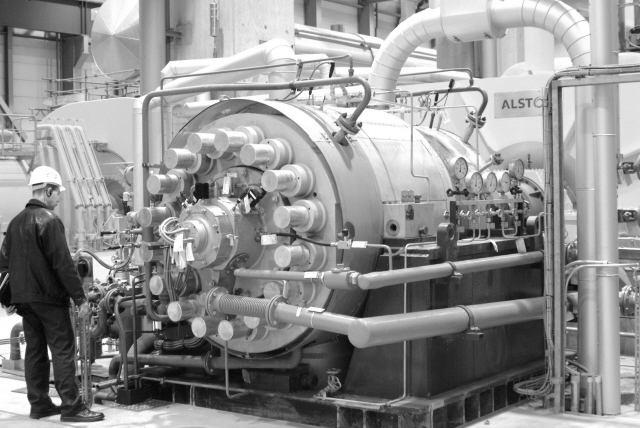
\includegraphics[height=8cm]{images/centrale_pompe_photo.jpg}
			\end{center}
			\supercaption{Photo d’une pompe du fabricant KSB menant \SI{2500}{\tonne\per\hour} d’eau à \SI{350}{\bar} dans une centrale à vapeur.\\
			Les pompes à liquide sont usuellement alimentées par un moteur électrique, mais ce modèle est alimenté mécaniquement par la turbine et doit ainsi fonctionner sur une plus grande plage de vitesses. Sa puissance maximale est de \SI{38}{\mega\watt} ; la puissance de la turbine entraînée dépasse \SI{800}{\mega\watt}.}{Photo \ccbysa \wcfile{Kesselspeisepumpe Kraftwerk Niederaussem.jpg}{KSB Aktiengesellschaft, Frankenthal}}
			\label{fig_centrale_pompe1}
		\end{figure}

		\begin{figure}
			\begin{center}
				
\includegraphics[height=4cm]{images/symbole_pompe.png}
			\end{center}
			\caption{Schéma de principe d’une pompe à eau.}
			\label{fig_centrale_pompe2}
		\end{figure}

		La puissance spécifique requise pour comprimer un débit de fluide d’une pression $p_A$ à une pression $p_B$, lorsque l’évolution est réversible, s’exprime à partir de la relation \ref{eq_travail_w_rév_so}. Comme le volume massique $v_L$  de l’eau liquide pure saturée (environ $v_L = \SI{1e-3}{\metre\cubed\per\kilogram}$) varie très peu avec sa pression, nous pouvons écrire :
		\begin{equation}
			{w}_\text{pompe~liquide} \approx v_L \int_\A^\B \diff p = v_L (p_\B - p_\A )
		\end{equation}

		\begin{description}
			\item dans le cas d’une pompe réversible à eau liquide.
		\end{description}

		 

	\subsection{Chaudière}
	\label{ch_chaudière}

		Dans les centrales à vapeur, les apports de chaleur se font à pression constante. L’eau du circuit thermodynamique est réchauffée par contact avec une autre canalisation : d’air dans le cas des centrales à combustion (déchets, charbon, gaz), ou d’eau (d’un circuit secondaire) dans le cas des centrales nucléaires%
		\footnote{Nous utilisons un deuxième circuit d’eau pour éviter de faire passer l’eau du circuit thermodynamique à haute pression dans le cœur même du réacteur.}\nolinebreak.

		L’extraordinaire comportement des fluides lorsqu’ils changent de phase tourne ici à notre avantage : en mélange di-phasique, une évolution à pression constante se fait aussi à température constante,\footnote{Bien revoir à ce propos le \courscinq.}
		ce qui nous permet de nous rapprocher des conditions prescrites par Carnot sans avoir recours à la moindre pièce mobile.
		
		Parce qu’elle fonctionne à haute pression (jusqu’à~\SI{60}{\bar} pour les installations modernes), et qu’elle est le théâtre de transferts de chaleur et gradients de température importants, la chaudière est un élément coûteux et lourd (figures~\ref{fig_centrale_chaudiere1} et~\ref{fig_centrale_chaudiere2}), même si son fonctionnement est simple.

		\begin{figure}
			\begin{center}
				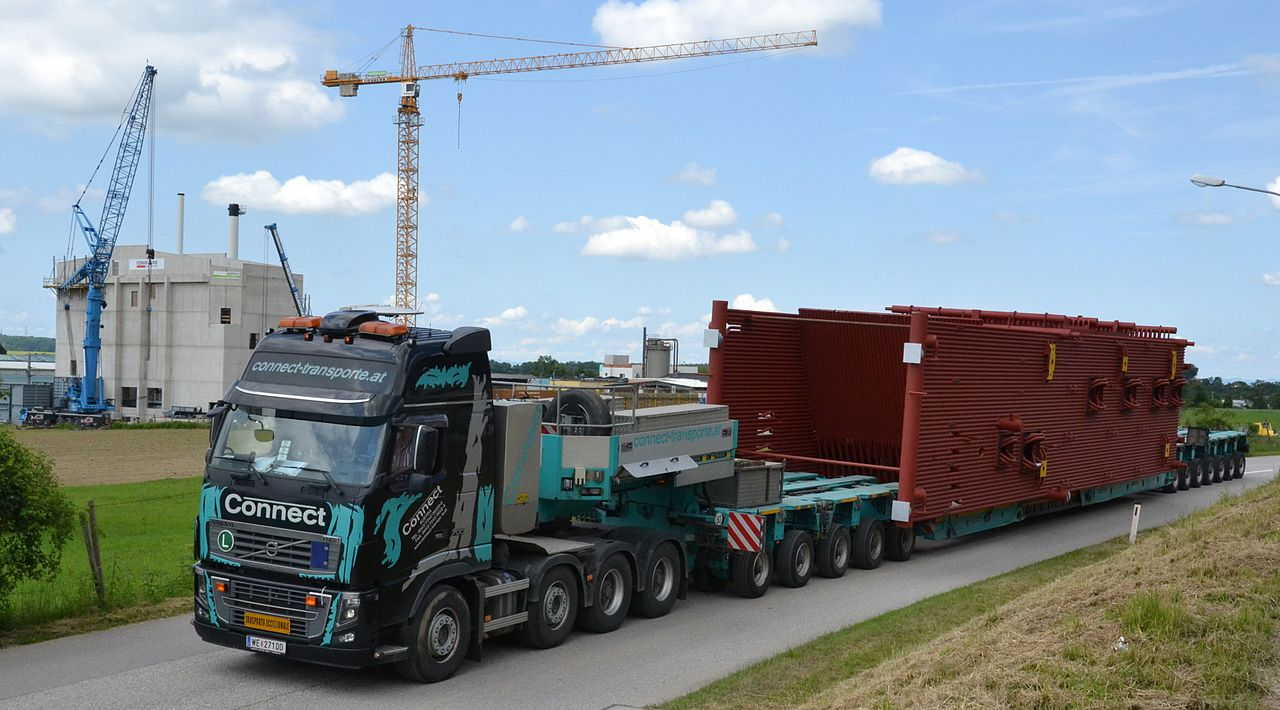
\includegraphics[width=\textwidth]{images/centrale_chaudiere_photo.jpg}
			\end{center}
			\supercaption{Transport d’une chaudière de centrale à bois capable de soutenir une pression de \SI{100}{\bar}.}{\wcfile{Antransport_Flossenwandkessel_Steyr.jpg}{Photo} \ccbysa par \wcu{Sensenschmied}}
			\label{fig_centrale_chaudiere1}
		\end{figure}

		\begin{figure}
			\begin{center}
				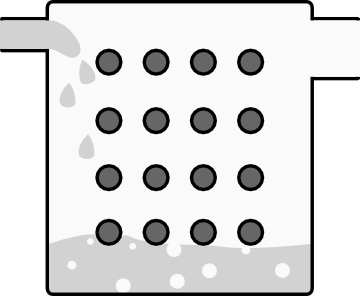
\includegraphics[width=4cm]{images/symbole_chaudiere.png}
			\end{center}
			\supercaption{Représentation schématique d’une chaudière.\\
		Dans une chaudière, l’eau pénètre à l’état liquide à gauche, et ressort en haut à droite à l’état de vapeur saturée. L’apport de chaleur est assuré par le contact avec les traverses des gaz de combustion.}{}
			\label{fig_centrale_chaudiere2}
		\end{figure}
		
		Lorsque la chaleur de la centrale provient d’une combustion, l’énergie thermique des gaz ne peut être transmise à l’eau du circuit que lorsque la température de cette dernière est plus faible. Ainsi, il est rejeté au-dessus de la chaudière une quantité de chaleur d’autant plus grande que la température minimale de l’eau y est haute. Le rendement d’une chaudière à gaz performante avoisine usuellement les \SI{80}{\percent}.

		Comme aucun travail mécanique n’est fourni à l’eau dans la chaudière, la puissance fournie par la chaudière à l’eau s’exprime selon :
		\begin{equation}
			\dot{Q}_\text{chaudière} = \dot{m} (h_2 - h_1)
		\end{equation}

		La différence de masse volumique entre les deux phases dans la chaudière fait qu’il est difficile de surchauffer la vapeur en présence de liquide\footnote{Le liquide, plus dense et donc au fond de la chaudière, est en effet plus à même d’absorber la chaleur à haute température.}\nolinebreak.
		Nous considérerons ainsi toujours que l’eau est sous forme de vapeur saturée (indice~$V$) à la sortie de la chaudière.

	\subsection{Turbine}

		La turbine (figures~\ref{fig_centrale_turbine1} et~\ref{fig_centrale_turbine2}) est la pièce maîtresse de toute centrale à vapeur. Longue de plusieurs dizaines de mètres dans les installations modernes, elle est équilibrée avec grand soin, mise en place dans son coffrage et, si elle fait l’objet d’attention adéquate (minimisation des gradients de température, lubrification avancée), peut délivrer de la puissance mécanique pendant plusieurs dizaines d’années sans interruption.

		\begin{figure}
			\begin{center}
				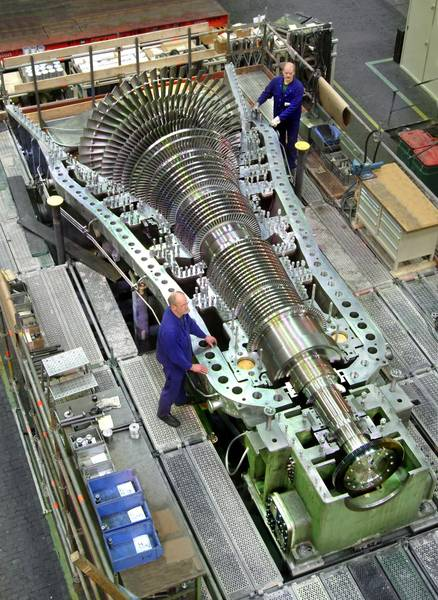
\includegraphics[height=9cm]{images/centrale_turbine_photo.jpg}
			\end{center}
			\supercaption{Turbine d’une centrale à vapeur de taille moyenne.\\
			Au fur et à mesure que l’eau traverse la turbine, elle perd de l’énergie sous forme de travail et son volume spécifique augmente, ce qui nécessite des pales toujours plus grandes.}{\wcfile{SteamTurbine.jpg}{Photo} \ccbysa MAN SE}
			\label{fig_centrale_turbine1}
		\end{figure}

		\begin{figure}
			\begin{center}
				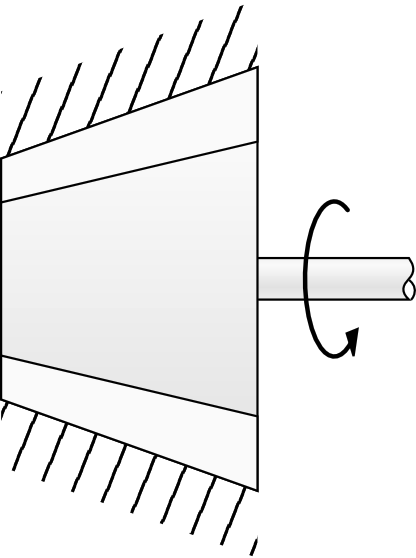
\includegraphics[width=4cm]{images/symbole_turbine.png}
			\end{center}
			\caption{Représentation schématique d’une turbine à vapeur.}
			\label{fig_centrale_turbine2}
		\end{figure}
		

		L’efficacité d’une turbine se mesure en comparant sa puissance avec celle d’une turbine idéale (une turbine qui serait isentropique). Nous nommons ce paramètre l’\vocab{efficacité isentropique} :
		\begin{equation}
			\eta_\text{T} \equiv  \frac{\dot{W}_\text{Turbine réelle}}{\dot{W}_\text{Turbine isentropique}}
			\label{def_efficacité_isentropique_turbine}
		\end{equation}
		
		\begin{equationterms}
			\item pour une turbine,
			\item où \tab $\dot{W}_\text{Turbine réelle}$ \tab\tab\tab est la puissance réelle fournie par la turbine,
			\item et \tab $\dot{W}_\text{Turbine isentropique}$ \tab la puissance d’une turbine isentropique fonctionnant avec le même débit de masse et entre les deux mêmes pressions.
		\end{equationterms}

		La puissance réelle, quant à elle, s’exprime toujours en fonction des propriétés du fluide à l’entrée et à la sortie de la turbine :
		\begin{equation}
			\dot{W}_\text{Turbine réelle} = \dot{m} (h_{2 \text{réel}} - h_1)
			\label{eq_puissance_turbine_vapeur}
		\end{equation}

		Avec une combinaison des équations~\ref{def_efficacité_isentropique_turbine} et~\ref{eq_puissance_turbine_vapeur}, on peut ainsi prévoir l’état de la vapeur à la sortie de n’importe quelle turbine dont on connaît la puissance et l’efficacité isentropique.

		Un paramètre important qui doit être surveillé est le titre de l’eau, en particulier dans les derniers étages. Les gouttelettes liquides, beaucoup plus denses que la vapeur qui les entoure, percutent en effet violemment les pales et en provoquent l’érosion. L’ingénieur/e thermodynamicien/ne veillera ainsi à garder un haut titre, usuellement sans descendre en deçà de~\SI{95}{\percent}.


	\subsection{Condenseur}

		Le condenseur (figures~\ref{fig_centrale_condenseur1} et~\ref{fig_centrale_condenseur2}), composant le moins glorieux de l’installation, est en charge de rejeter toute la chaleur dont l’ingénieur/e ne sait plus faire usage\footnote{On relira, pour comprendre l’inéluctabilité de ce rejet phénoménal, le \courssept.}. L’eau y est toujours refroidie à pression constante, ce qui ne nécessite pas de pièce mobile.

		\begin{figure}
			\begin{center}
				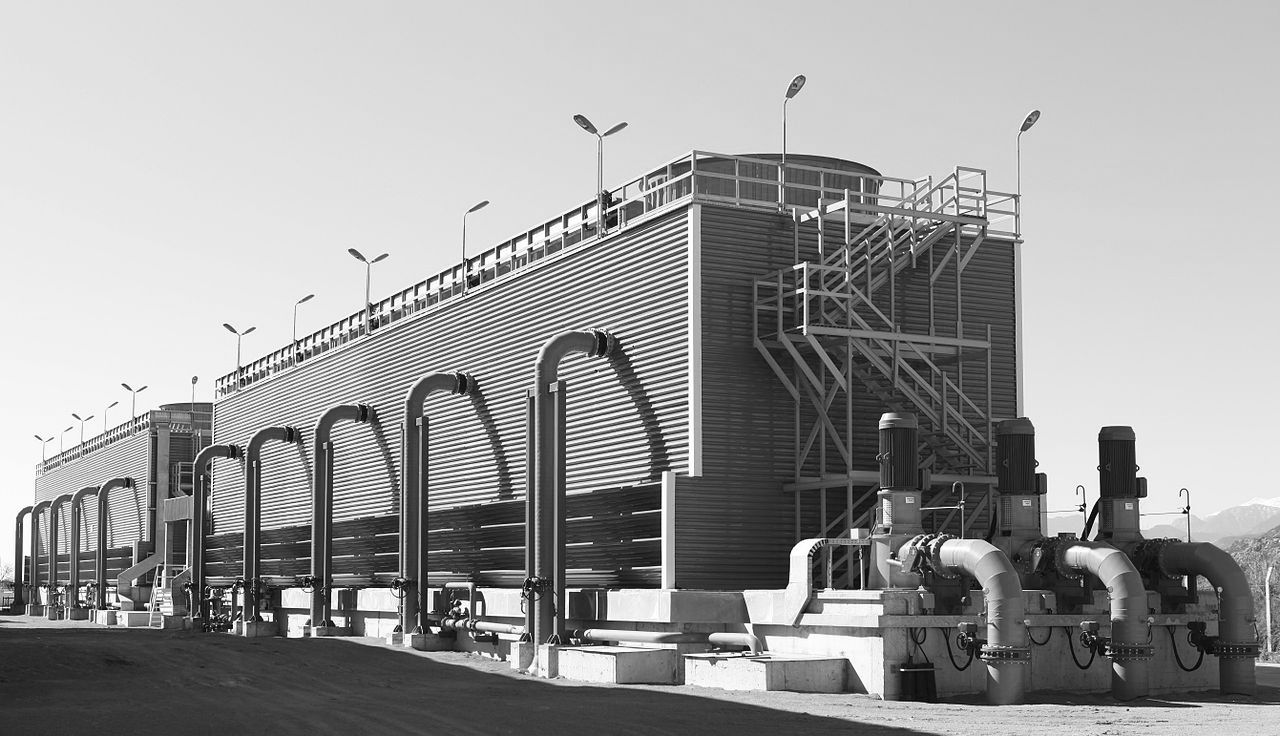
\includegraphics[width=\textwidth]{images/centrale_condenseur_photo.jpg}
			\end{center}
			\supercaption{Condenseur avec cheminées de refroidissement intégrées.}{\wcfile{Cenk_Endustri_Field_Erected_Industrial_Cooling_Tower.JPG}{Photo} \ccbysa Cenk Endustri}
			\label{fig_centrale_condenseur1}
		\end{figure}

		\begin{figure}
			\begin{center}
				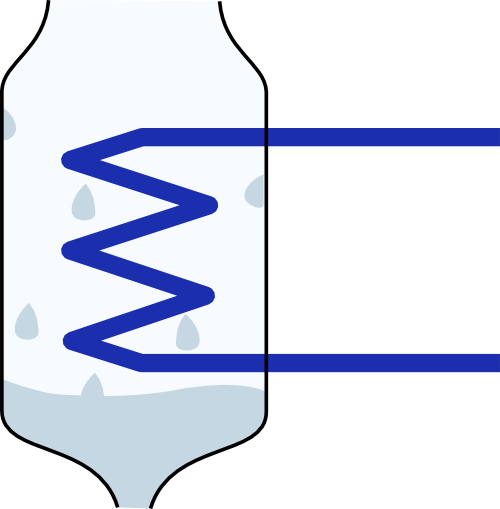
\includegraphics[width=4cm]{images/symbole_condenseur.png}
			\end{center}
			\supercaption{Représentation schématique d’un condenseur.\\
			L’eau du circuit thermodynamique y pénètre par le haut, dans un état proche de la vapeur saturée. Elle en ressort par le bas à l’état liquide. L’extraction de chaleur est usuellement assurée par un circuit d’eau secondaire (schématisé en bleu) qui est mise en contact avec l’atmosphère.}{}
			\label{fig_centrale_condenseur2}
		\end{figure}

		Technologiquement, c’est un élément simple : on met la canalisation de vapeur en contact avec un circuit de température basse. Usuellement, ce circuit de refroidissement est constitué d’eau extérieure provenant d’une rivière ou de la mer,\footnote{Il y a deux intérêts à l’utilisation d’un circuit de refroidissement secondaire. D’une part, on peut abaisser la pression dans le condenseur plus bas que la pression atmosphérique et ainsi réduire la température minimale du cycle. D’autre part, l’eau du circuit thermodynamique, épurée au prix d’efforts considérables, n’est pas perdue dans l’atmosphère.}
		qui sera refroidie ensuite par évaporation dans les larges cheminées que l’on aperçoit aux abords des centrales. Comme la pression de la vapeur à l’intérieur du condenseur est souvent très basse (jusqu’à~\SI{1}{\bar}) pour abaisser la température minimale du cycle de la centrale, il faut veiller à l’étanchéité du condenseur pour éviter que de l’air ou de l’eau extérieurs ne s’insèrent dans le circuit principal.

		La puissance perdue par la vapeur dans le condenseur s’exprime selon :
		\begin{equation}
			\dot{Q}_\text{condenseur} = \dot{m} (h_2 - h_1)
		\end{equation}





\section{Cycles moteurs à vapeur}



	\subsection{Le cycle de Carnot}

		Comme la température d’un mélange liquide-vapeur reste constante lorsqu’on le chauffe à pression constante, la réalisation d’échanges de chaleur isotherme (caractéristique importante du cycle de Carnot) est relativement aisée avec la vapeur. Une machine à vapeur basée sur un cycle de Carnot est schématisée en figures~\ref{fig_machine_vapeur_carnot} et~\ref{fig_ts_machine_vapeur_carnot}.


		\begin{figure}
			\begin{center}
				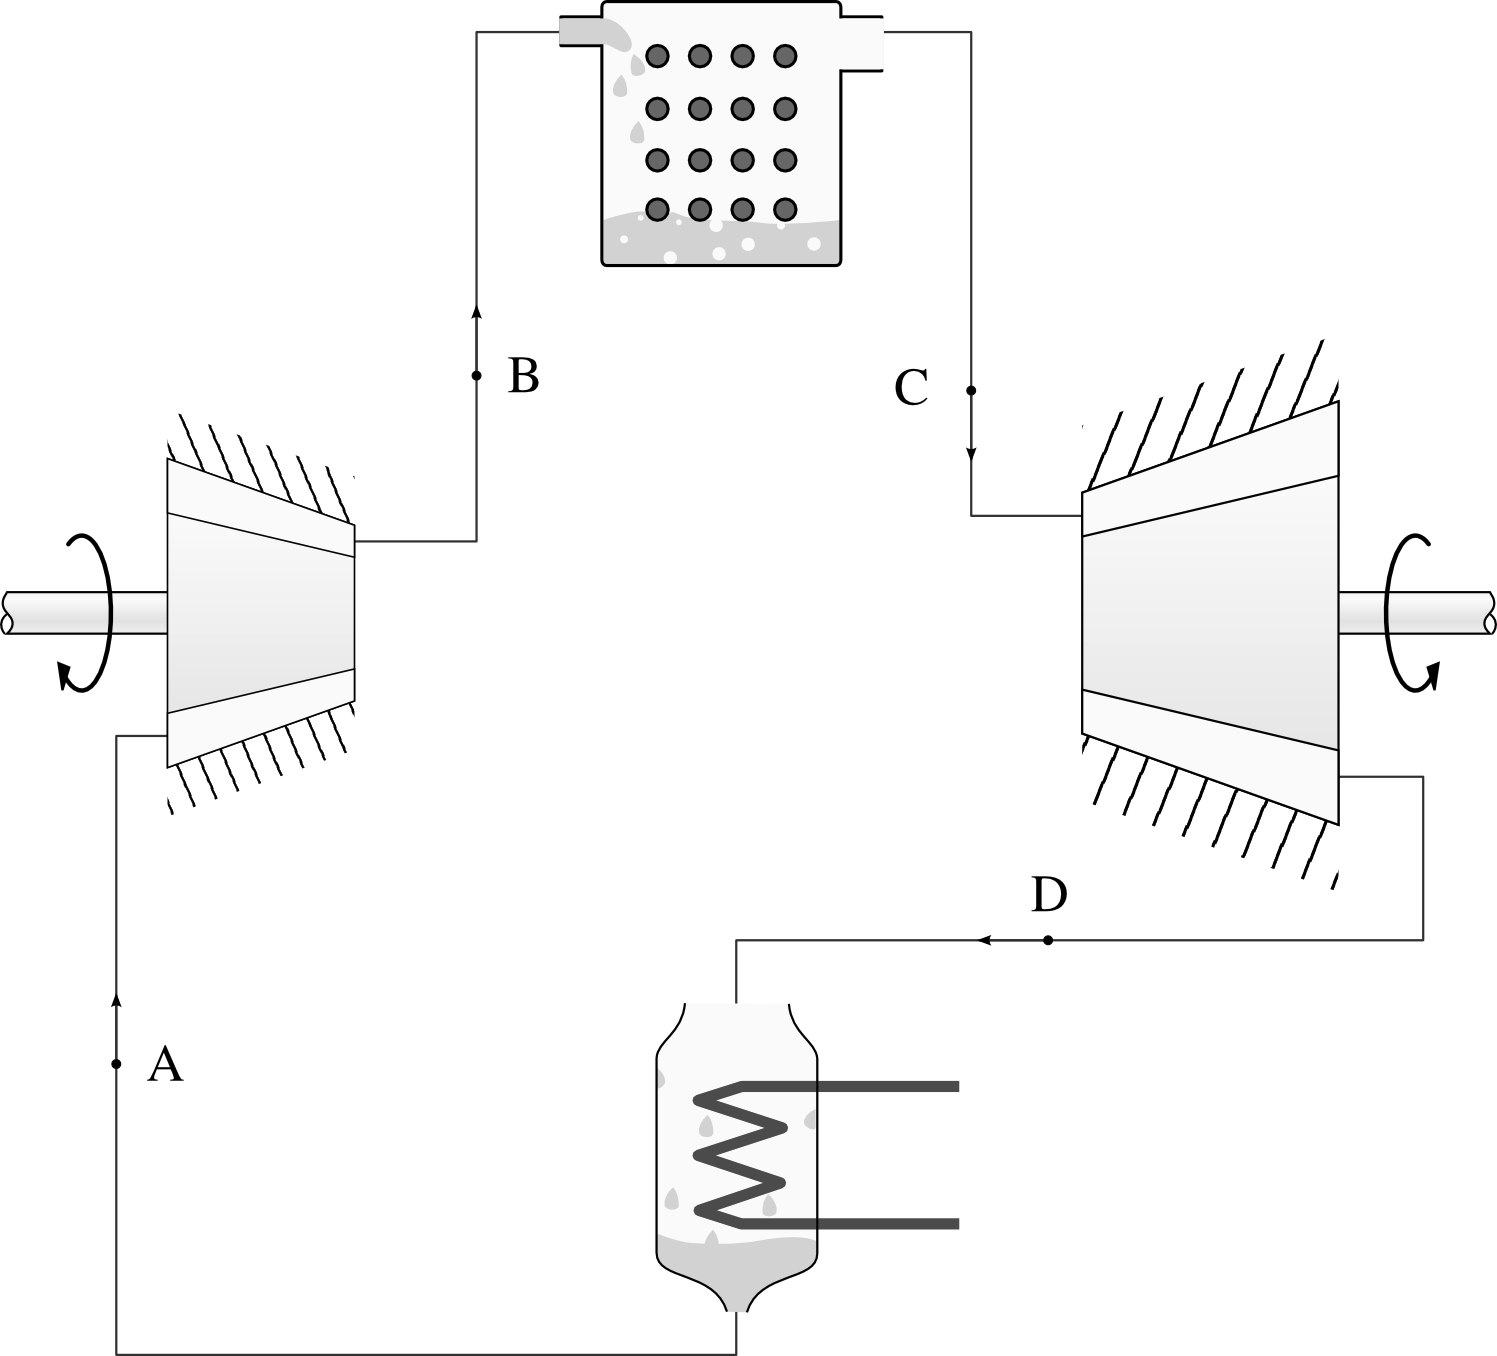
\includegraphics[height=11cm]{images/circuit_carnot_lv.png}
			\end{center}
			\caption{Circuit d’une centrale à vapeur fonctionnant sur un cycle de Carnot.}
			\label{fig_machine_vapeur_carnot}
		\end{figure}

		\begin{figure}
			\begin{center}
				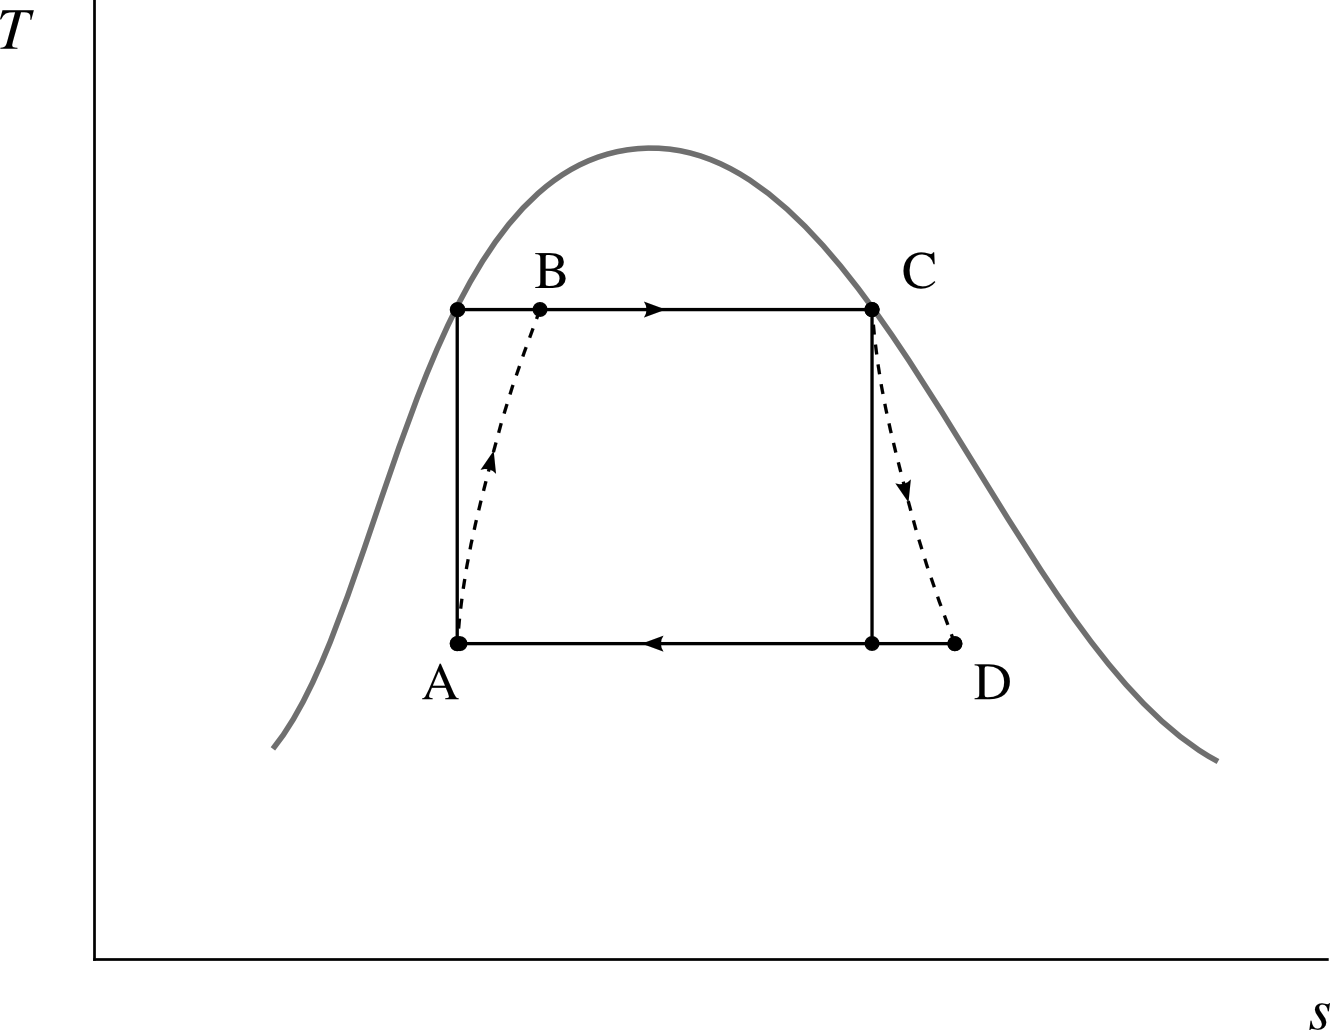
\includegraphics[width=10cm]{images/ts_lv_carnot.png}
			\end{center}
			\caption{Diagramme température-entropie d’une centrale à vapeur fonctionnant sur un cycle de Carnot. Les trajets en pointillés représentent les évolutions réelles (irréversibles) du fluide pendant les compressions et détentes.}
			\label{fig_ts_machine_vapeur_carnot}
		\end{figure}

		L’efficacité du cycle moteur de Carnot (\ref{eq_efficacité_moteur_carnot_température}) n’est atteinte que lorsque la turbine et le compresseur fonctionnent de façon isentropique. En pratique, comme nous l’avons vu, la puissance de la turbine est toujours plus faible et celle du compresseur toujours plus grande qu’elles ne pourraient l’être.
		
		Si l’on connaît l’efficacité isentropique $\eta _T$ de la turbine (\ref{def_efficacité_isentropique_turbine}), on peut exprimer sa puissance en fonction des propriétés de la vapeur :
		\begin{equation}
			w_\text{Turbine~réelle} = w_{\C \to \D_\text{réel}} = (h_{\D_\text{réel}} - h_\C) = \eta_\text{T} \ (h_{\text{D'}} - h_\C)
		\end{equation}

	\subsection{Le cycle de Rankine}
	\label{ch_cycle_de_rankine}

		En pratique, l’utilisation du cycle de Carnot comme ci-haut pose plusieurs difficultés :

		\begin{itemize}
			\item La compression d’un mélange di-phasique est technologiquement difficile (\S\ref{ch_moteurs_vapeur_compresseurs_et_pompes}) ;
			\item Dans le condenseur, il est difficile d’interrompre la condensation à un endroit précis (le point A en figures~\ref{fig_machine_vapeur_carnot} et~\ref{fig_ts_machine_vapeur_carnot} plus haut, dont le titre est proche mais différent de~0).
		\end{itemize}

		\wed{William John Macquorn Rankine}{William Rankine}, ingénieur anglo-saxon digne de ses compatriotes, propose en 1859 une modification du cycle en poursuivant la condensation jusqu’à saturation et en ne compressant l’eau qu’à l’état liquide. Une machine basée sur ce cyle est décrite en figures~\ref{fig_cycle_rankine} et~\ref{fig_ts_lv_rankine}.

		\begin{figure}
			\begin{center}
				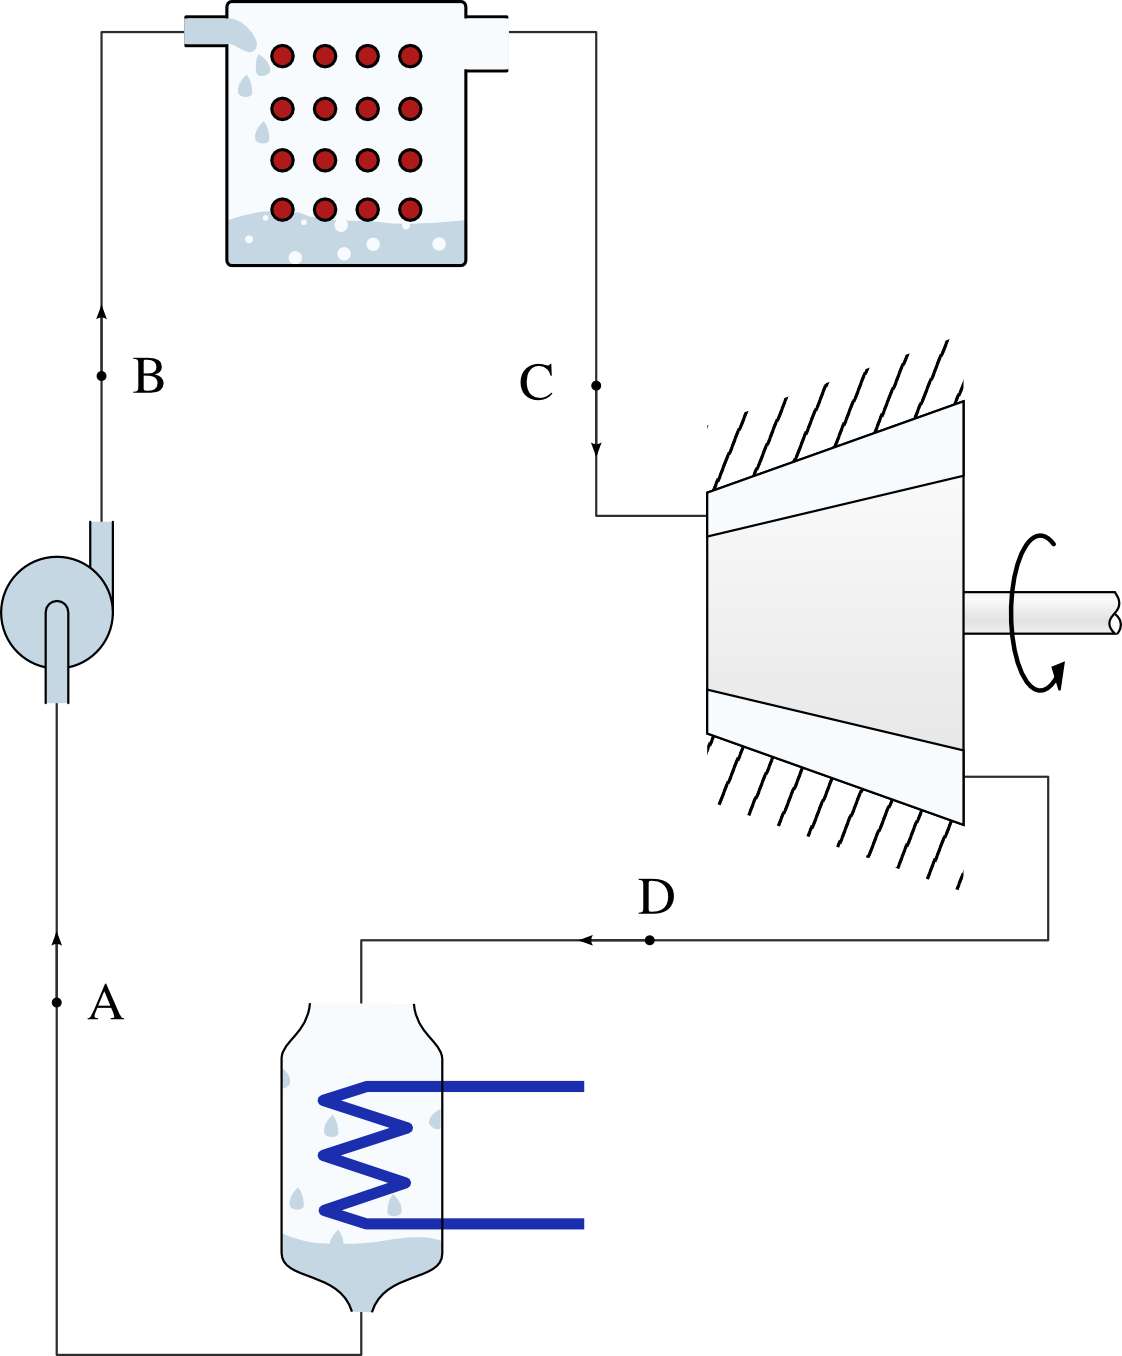
\includegraphics[height=11cm]{images/circuit_rankine.png}
			\end{center}
			\caption{Circuit d’une centrale à vapeur fonctionnant sur un cycle de Rankine. L’eau à la sortie du condenseur est sous forme de liquide saturée ; elle rentre dans la chaudière à plus faible température.}
			\label{fig_cycle_rankine}
		\end{figure}

		\begin{figure}
			\begin{center}
				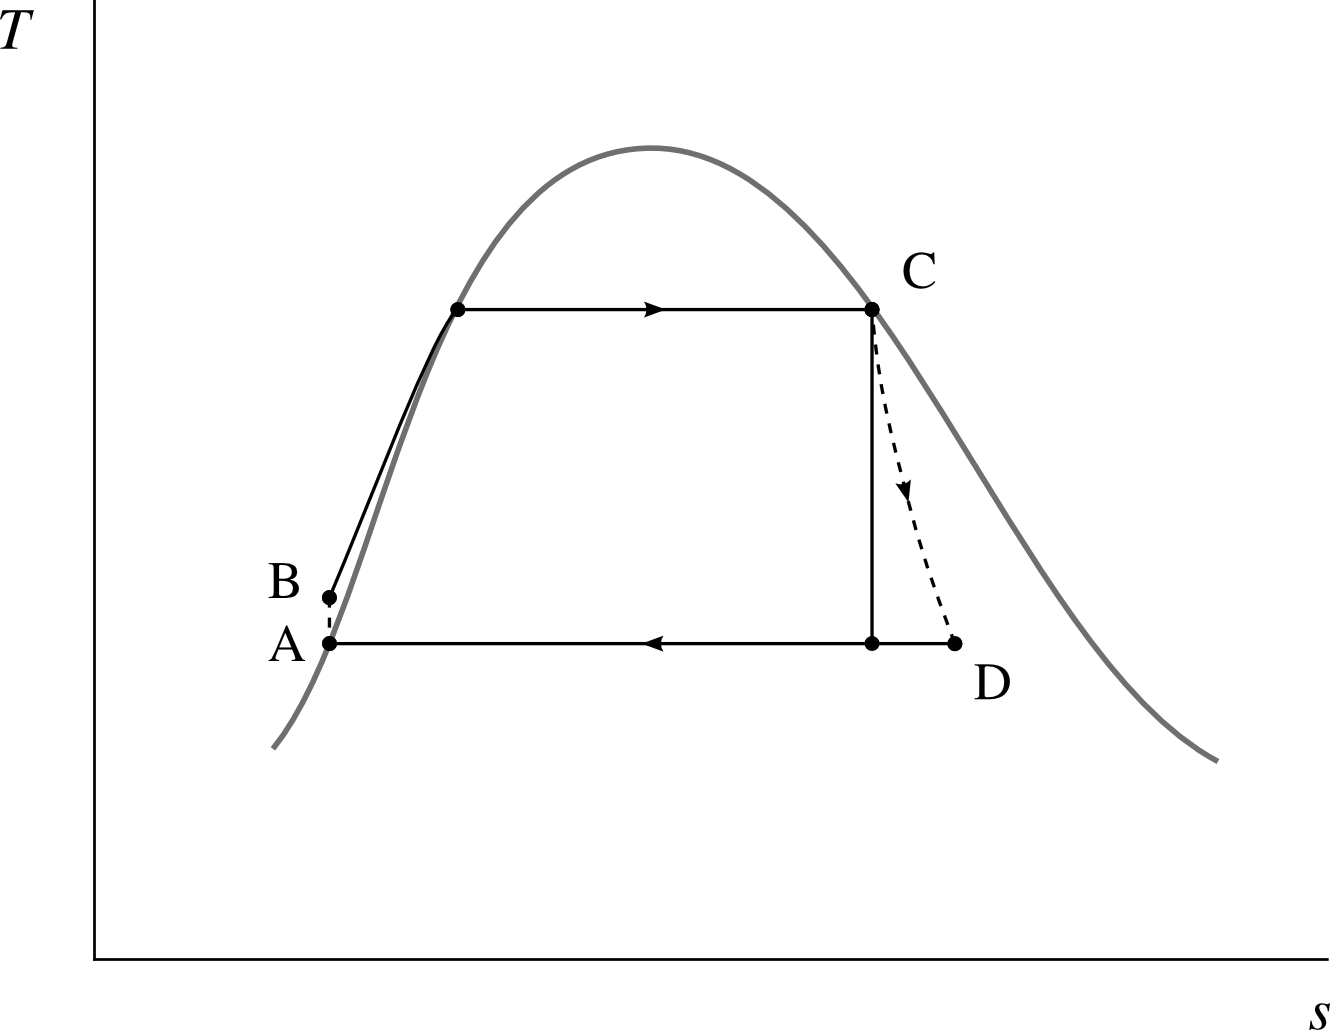
\includegraphics[width=10cm]{images/ts_lv_rankine.png}
			\end{center}
			\caption{Diagramme température-entropie d’une centrale à vapeur fonctionnant sur un cycle de Rankine.}
			\label{fig_ts_lv_rankine}
		\end{figure}

		Le \vocab{cycle de Rankine} utilise donc une pompe à eau liquide plutôt qu’un compresseur en mélange liquide/vapeur. Technologiquement, une pompe est plus simple à concevoir, fabriquer, et opérer qu’un compresseur. Autre avantage, la compression d’un liquide est plusieurs dizaines de fois plus économe en énergie que celle du mélange (\S\ref{ch_moteurs_vapeur_compresseurs_et_pompes}). 
		
		Toutefois, cette économie d’énergie n’est pas sans contrepartie : à la sortie de la pompe (point B), l’eau est à température bien plus faible qu’elle ne l’était à la sortie du compresseur en \cref{fig_machine_vapeur_carnot}. C’est \emph{la chaudière} qui devra ramener l’eau à l’état de liquide saturé. Autrement dit, il faut fournir une dépense supplémentaire considérable sous forme de chaleur pour compenser la baisse de puissance de compression.

		On peut remarquer qu’une partie importante de la chaleur apportée par la chaudière (c’est-à-dire $q_\text{ch.} = h_\C - h_B$ ) n’est plus apportée à température constante. Nous avons vu aux chapitres~\sept et~\huit qu’un apport de chaleur à basse température se traduit toujours par un rendement plus faible.\\
		Toutefois, en pratique, cet apport de chaleur peut rendre possible l’exploitation de sources de chaleur à basse température, comme les gaz d’échappement rejetés au-dessus de la chaudière. Ainsi, dans certains cas, la chute du rendement thermodynamique ($\eta_\text{moteur}$) peut être compensée par une augmentation du rendement de la chaudière ($\eta_\text{chaudière}$), qui peut extraire plus d’énergie au combustible pour le transmettre à la vapeur.
		
		Rankine s’est ainsi écarté volontairement du cycle de Carnot, et a ce faisant réduit le rendement thermodynamique global (même si cette baisse peut souvent être compensée par une augmentation du rendement de la chaudière). Par contre, en faisant disparaître le compresseur, sa modification permet de réduire fortement la taille et la complexité de l’installation.

		 

	\subsection{La surchauffe}

		Pour réduire la consommation spécifique ($SSC$) d’une centrale, il est souhaitable d’augmenter la puissance développée par la turbine pour un débit de vapeur donné. Pour cela, il existe plusieurs options :

		\begin{itemize}
			\item Augmenter l’enthalpie à l’entrée de la turbine (c’est-à-dire augmenter la pression de saturation dans la chaudière). \\
			Malheureusement, cela impose à la chaudière d’être plus résistante et plus coûteuse ; et de plus, cela réduit la quantité de chaleur spécifique qu’il est possible d’y apporter, puisque l’enthalpie de vaporisation $h_{LV}$ décroît avec la température ;

			\item Réduire l’enthalpie à la sortie de la turbine (c’est-à-dire diminuer la pression dans le condenseur). \\
			Cela nécessite une turbine de plus grande taille,  favorise l’insertion de bulles d’air dans le circuit de vapeur, et surtout, réduit le titre de l’eau en sortie de turbine ;

			\item Augmenter l’enthalpie (et donc la température de la vapeur) \emph{après} sa sortie de la chaudière.\\
			Cela permet  d’utiliser pleinement les capacités de la turbine, dont les limites métallurgiques (généralement autour de~\SI{1000}{\kelvin}) dépassent déjà souvent celles des chaudières.
		\end{itemize}

		C’est cette dernière option qui est très souvent choisie. On nomme cette modification la \vocab{surchauffe} : la vapeur est surchauffée à la sortie de la chaudière%
		\footnote{La surchauffe pourrait théoriquement être effectuée dans la chaudière même ; cependant, la densité de la vapeur surchauffée étant relativement faible, il est plus aisé de la mettre en contact avec les gaz les plus chauds en dehors (et en dessous) de la chaudière.}, à pression constante, à travers une série de tubes portés à plus haute température (figures~\ref{fig_cycle_rankine_surchauffe} et~\ref{fig_ts_lv_rankine_surchauffe}).

		\begin{figure}
			\begin{center}
				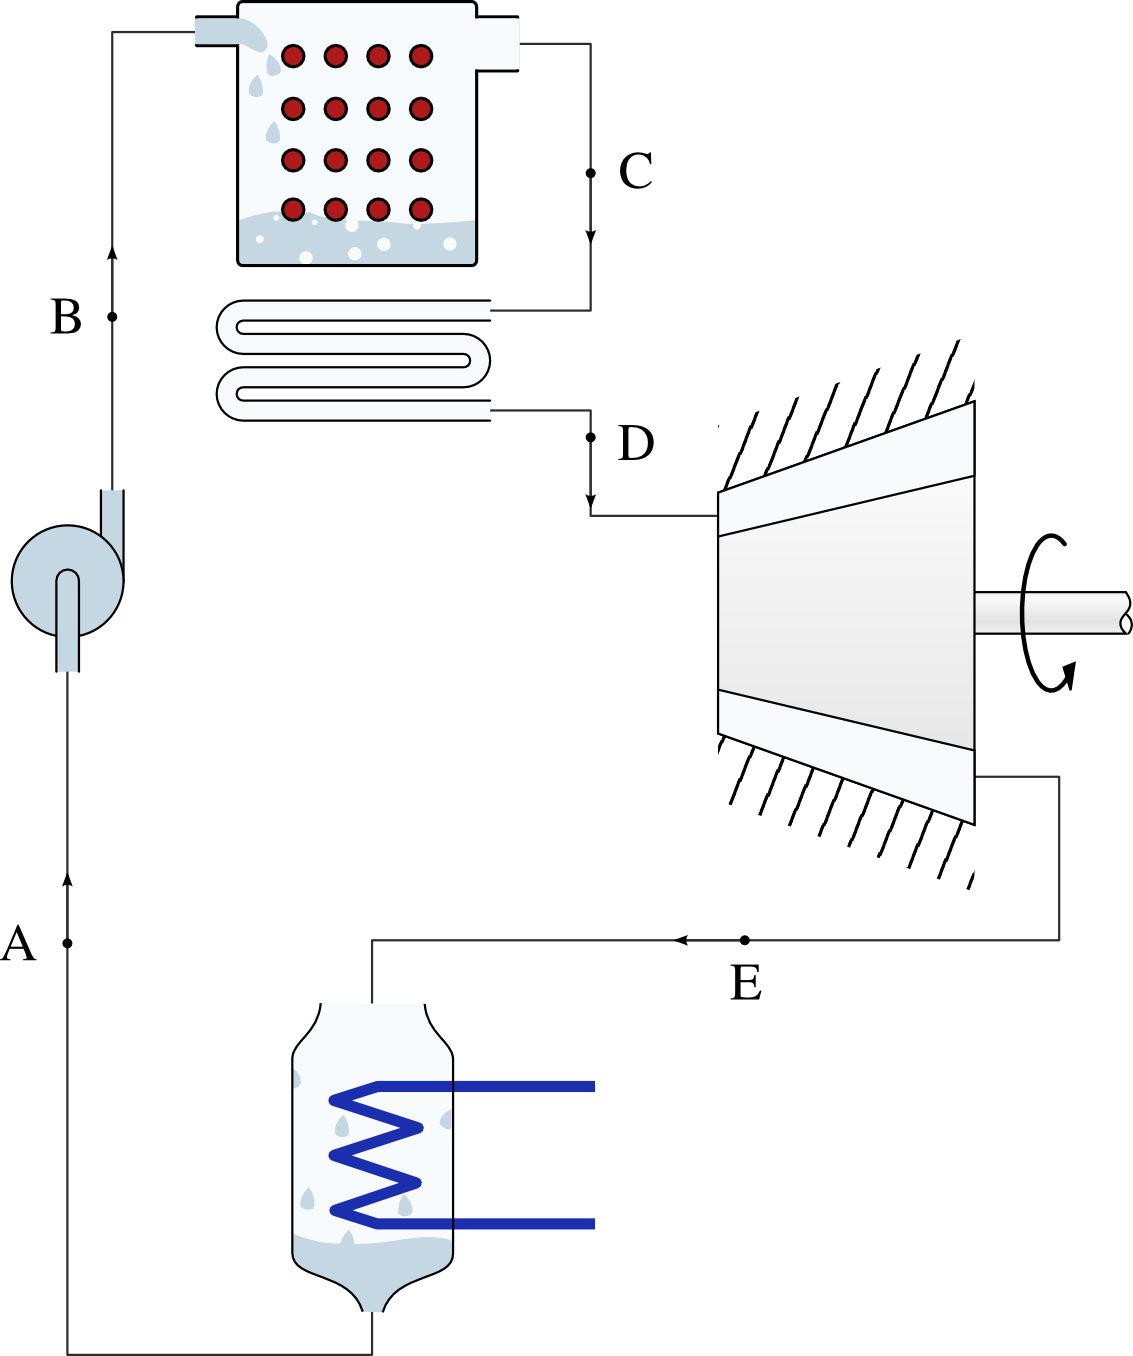
\includegraphics[height=11cm]{images/circuit_rankine_surchauffe.png}
			\end{center}
			\caption{Circuit d’une centrale à vapeur fonctionnant sur un cycle de Rankine surchauffé. L’eau à la sortie de la chaudière est portée à plus haute température (section C $\rightarrow $ D) avant de pénétrer dans la turbine.}
			\label{fig_cycle_rankine_surchauffe}
		\end{figure}

		\begin{figure}
			\begin{center}
				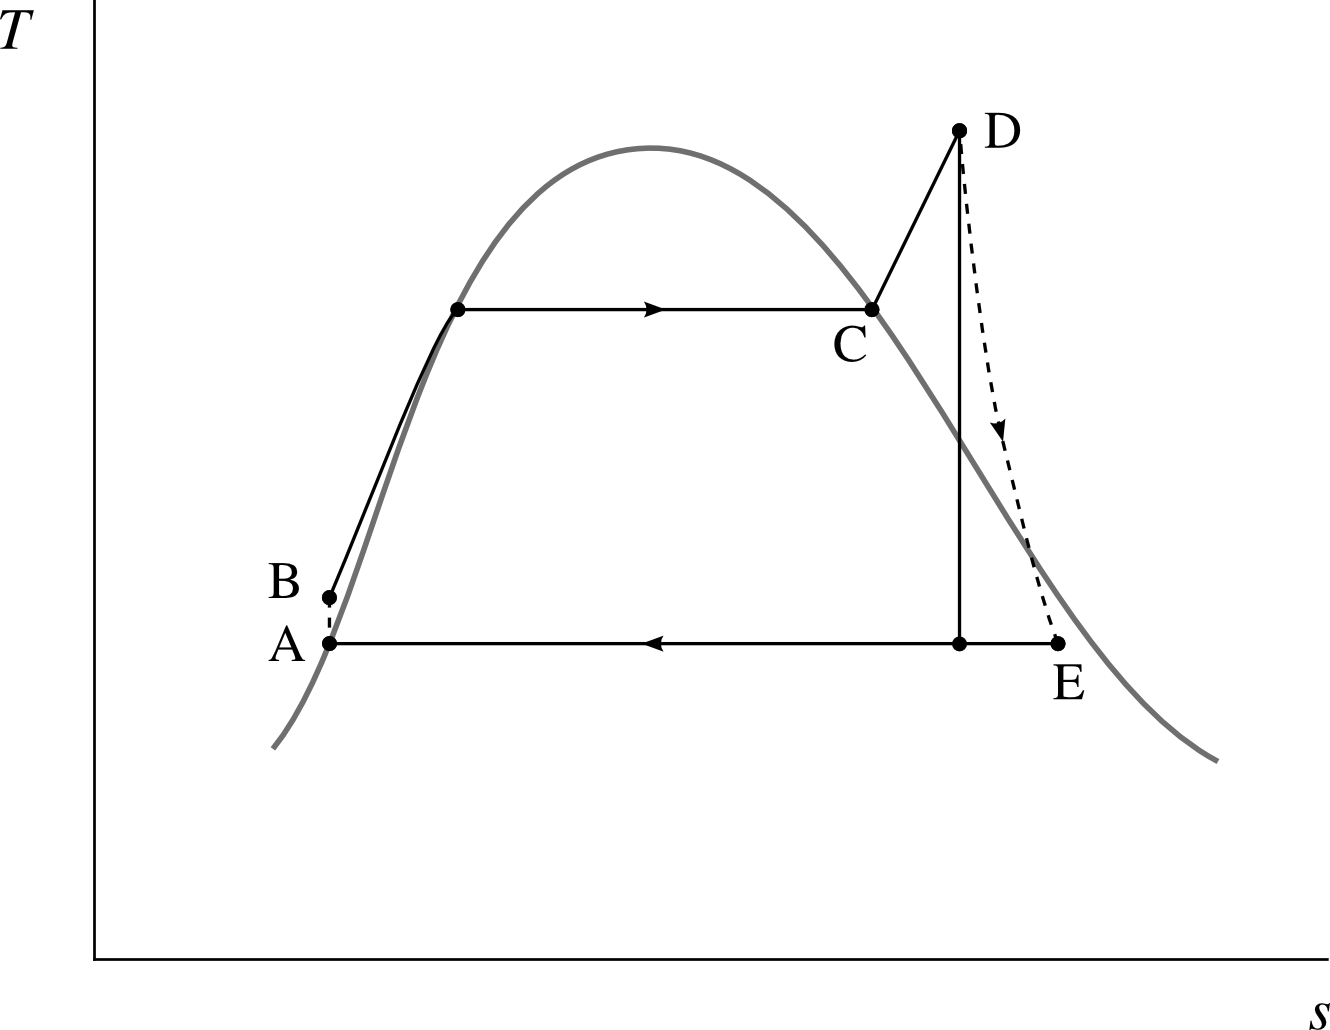
\includegraphics[width=10cm]{images/ts_lv_rankine_surchauffe.png}
			\end{center}
			\caption{Diagramme température-entropie d’une centrale à vapeur fonctionnant sur un cycle de Rankine surchauffé.}
			\label{fig_ts_lv_rankine_surchauffe}
		\end{figure}

		L’avantage principal de la modification est la diminution de la consommation spécifique : la puissance fournie est augmentée pour un débit de vapeur donné, grâce à une modification relativement peu complexe à mettre en œuvre. Autre avantage, l’augmentation de la température moyenne à laquelle la chaleur est apportée tend à augmenter le rendement thermodynamique. Enfin, il devient possible de décaler la plage d’utilisation de la turbine entièrement dans le domaine de la vapeur surchauffée : l’érosion des pales par l’eau liquide est ainsi évitée.


	\subsection{La resurchauffe}
	\label{ch_resurchauffe}

		Pour augmenter à nouveau la puissance de l’installation sans augmenter le débit de vapeur (et donc sa taille globale et le coût de la chaudière), il est possible de chauffer une deuxième fois la vapeur avant sa sortie de la turbine (figures~\ref{fig_cycle_resurchauffe} et~\ref{fig_ts_lv_surchauffe_resurchauffe}). C’est ce que l’on appelle la \vocab{resurchauffe}.

		\begin{figure}
			\begin{center}
				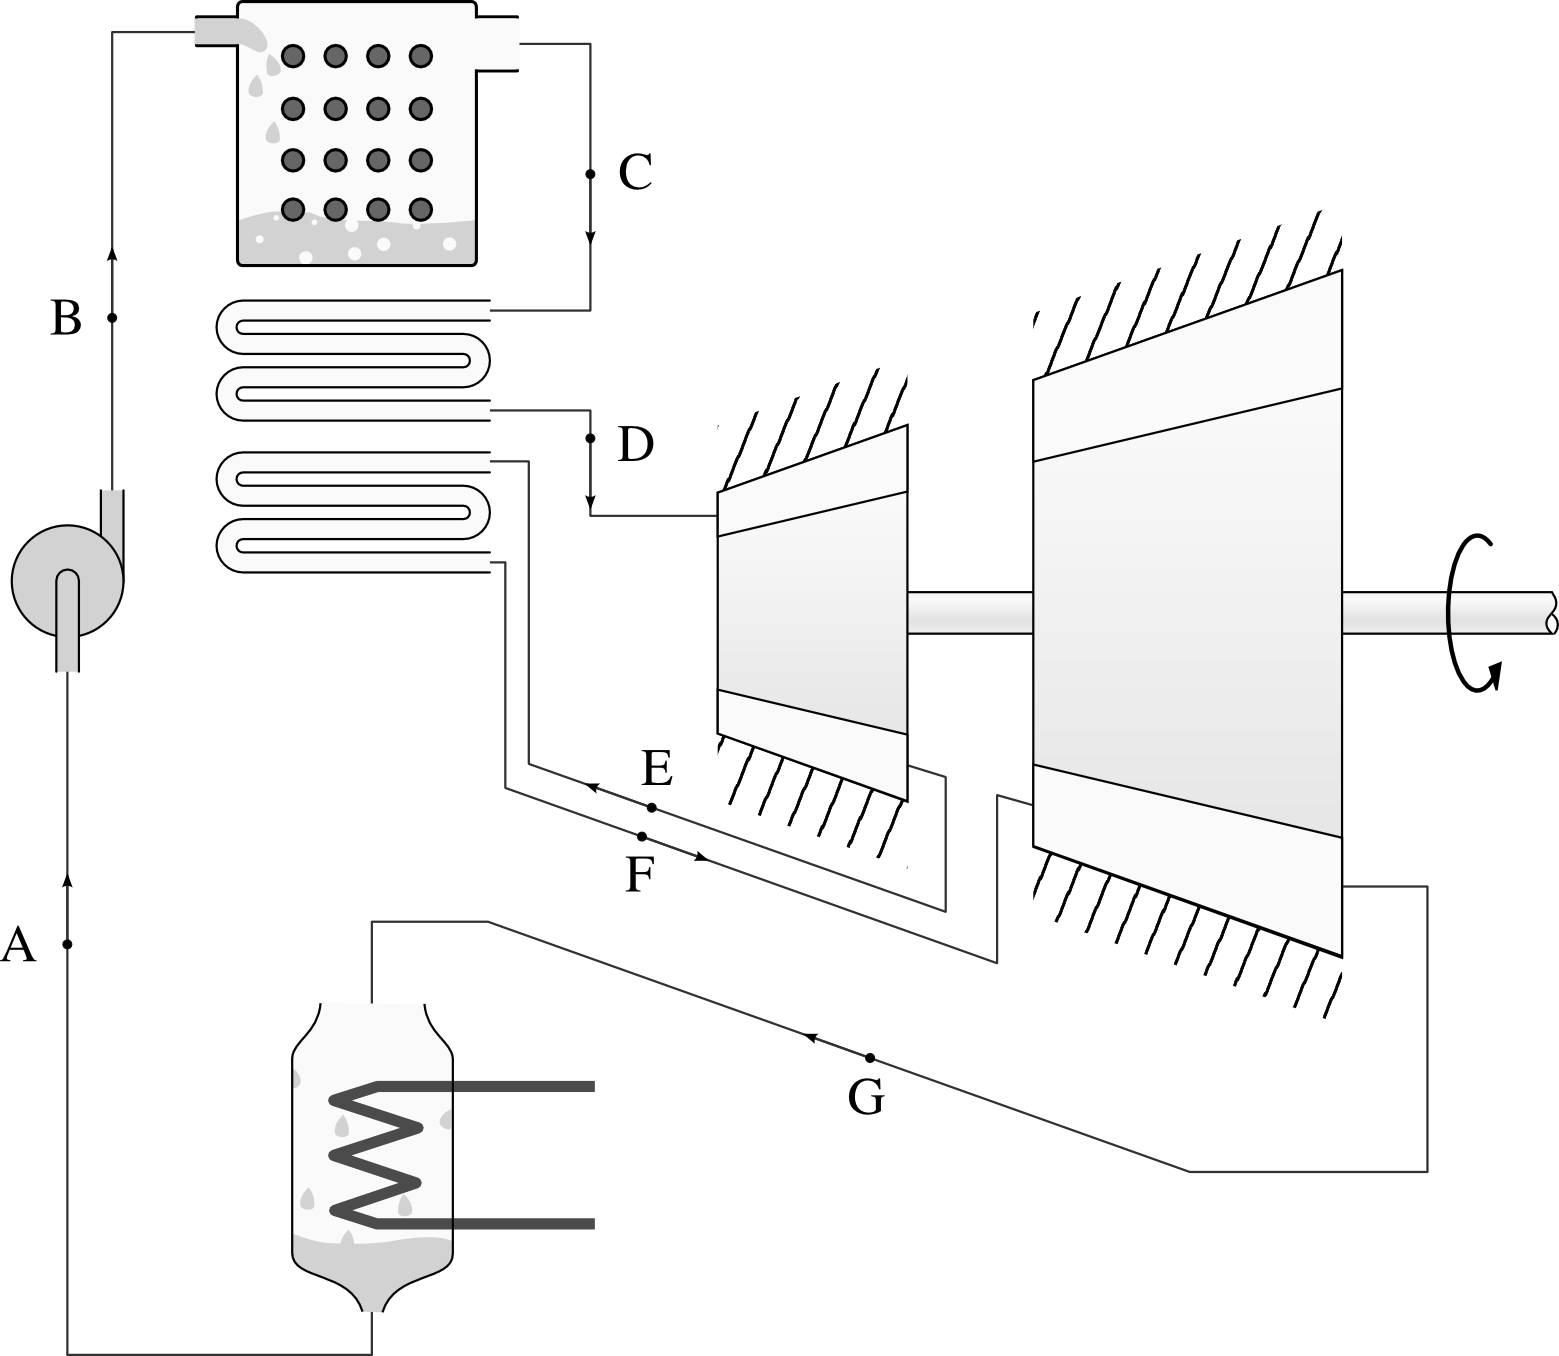
\includegraphics[height=11cm]{images/circuit_surchauffe_resurchauffe.png}
			\end{center}
			\caption{Circuit d’une centrale à vapeur fonctionnant sur un cycle de Rankine resurchauffé.}
			\label{fig_cycle_resurchauffe}
		\end{figure}

		\begin{figure}
			\begin{center}
				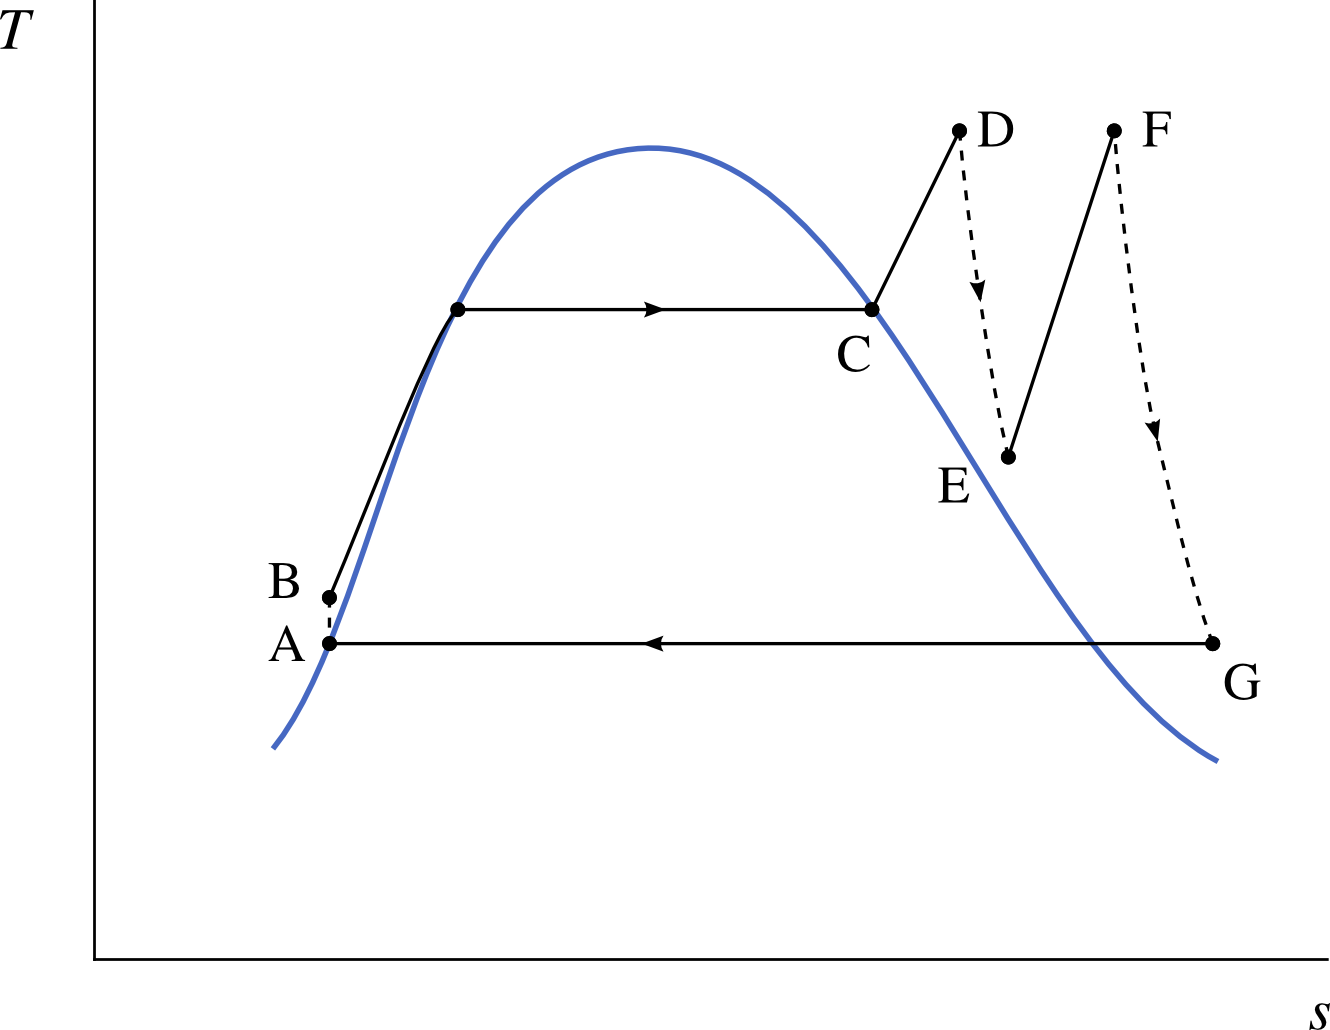
\includegraphics[width=10cm]{images/ts_lv_rankine_surchauffe_resurchauffe.png}
			\end{center}
			\caption{Diagramme température-entropie d’une centrale à vapeur fonctionnant sur un cycle de Rankine resurchauffé.}
			\label{fig_ts_lv_surchauffe_resurchauffe}
		\end{figure}

		Avec cette modification, la détente dans la turbine est interrompue ; et la vapeur est conduite dans une nouvelle série de tubes pour porter à nouveau sa température à haute température (usuellement aux limites métallurgiques de la turbine). La détente est alors complétée jusqu’à la pression du condenseur.

		Le rendement global de l’installation est augmenté si la température moyenne de chauffage l’est aussi ; il faut donc choisir avec soin la pression de la resurchauffe. La consommation spécifique, elle, est diminuée dans tous les cas, avec les avantages décrits plus haut.



	\subsection{La régénération}

		Lorsque Rankine a modifié le cycle de Carnot, il a réduit le travail fourni pour compresser l’eau, et augmenté la chaleur nécessaire pour l’amener en entrée de turbine. En contrepartie, le rendement thermodynamique a diminué : en effet, lorsque l’eau pénètre dans la chaudière, sa température est faible. Elle reçoit de la chaleur de façon non-réversible.

		Pour augmenter la réversibilité du cycle (et donc son rendement), il est possible de réchauffer l’eau progressivement, en utilisant la chaleur en provenance de la turbine (où la température de la vapeur varie). Cette technique est nommée \vocab{régénération}. On peut ainsi imaginer un cycle comme décrit en figures~\ref{fig_circuit_regeneration} et~\ref{fig_ts_lv_regeneration} ci-dessous, où l’eau liquide en sortie de pompe est réchauffée progressivement en refroidissant la turbine.

		\begin{figure}
			\begin{center}
				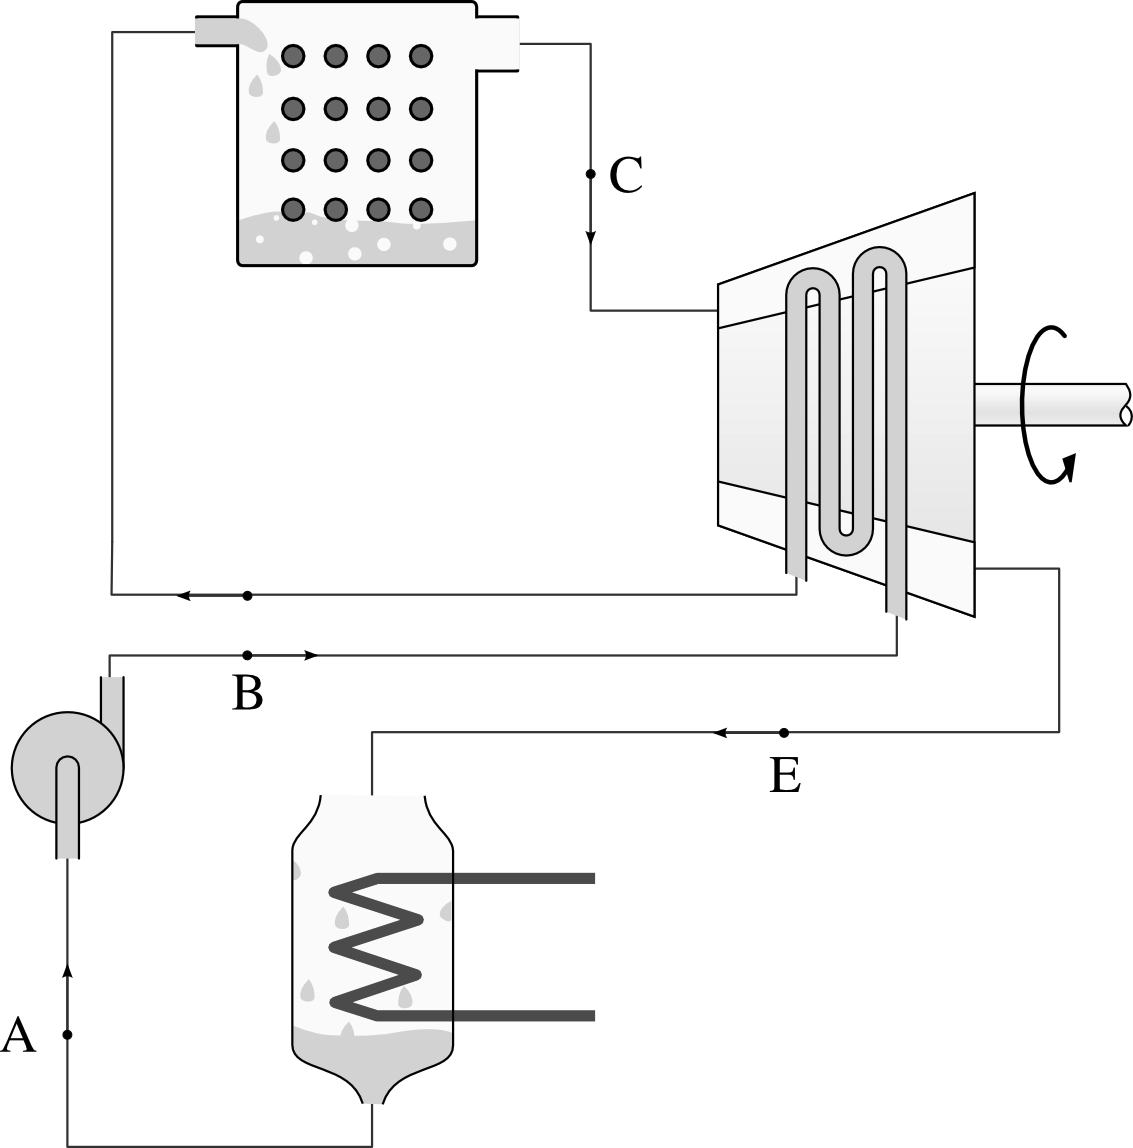
\includegraphics[height=11cm]{images/circuit_regeneration.png}
			\end{center}
			\caption{Circuit d’une centrale à vapeur avec régénération. On prélève de la chaleur à la turbine pour réchauffer l’eau liquide avant qu’elle ne pénètre dans la chaudière. Idéalement, l’échange de chaleur se fait de façon réversible.}
			\label{fig_circuit_regeneration}
		\end{figure}

		\begin{figure}
			\begin{center}
				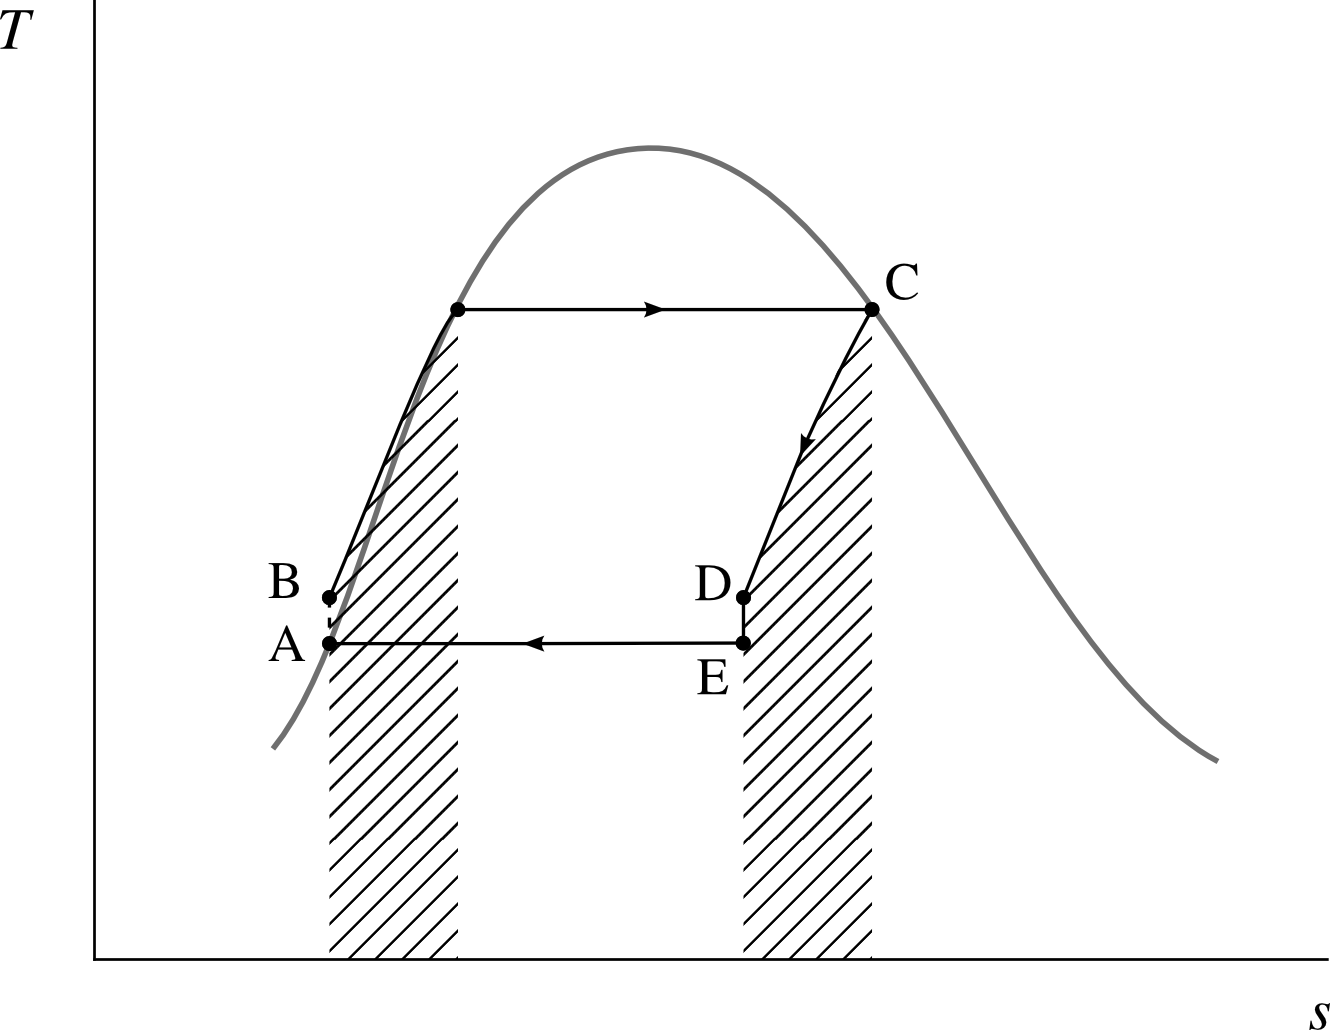
\includegraphics[width=10cm]{images/ts_lv_regeneration.png}
			\end{center}
			\caption{Diagramme température-entropie d’une centrale à vapeur avec régénération.}
			\label{fig_ts_lv_regeneration}
		\end{figure}


		Dans le cas limite où toute la chaleur utilisée lors de la régénération est transmise avec une différence de température infiniment faible, le cycle est réversible et le rendement du moteur de Carnot est atteint%
			\footnote{Cela est vrai même si le cycle ne suit pas à proprement parler le cycle de Carnot. Il suffit qu’il soit parfaitement réversible.}\nolinebreak.

		En pratique hélas, un tel dispositif est difficile à réaliser. En effet, la transmission réversible de chaleur est complexe à mettre en place dans la turbine, élément dont la conception et la fabrication sont déjà très coûteuses. De plus, le refroidissement de la vapeur réduit son titre, augmentant la quantité d’eau liquide érodant les pièces de la turbine.

		Pour mettre en place la régénération, on a donc recours à la technique de \vocab{prélèvement turbine}. De la vapeur est ponctionnée depuis la turbine, et mélangée à l’eau liquide en sortie de pompe (figures~\ref{fig_cycle_prélèvement_vapeur} et~\ref{fig_ts_lv_prelevement_vapeur}). On obtient ainsi un transfert de chaleur qu’il est aisé de mettre en œuvre.

		\begin{figure}
			\begin{center}
				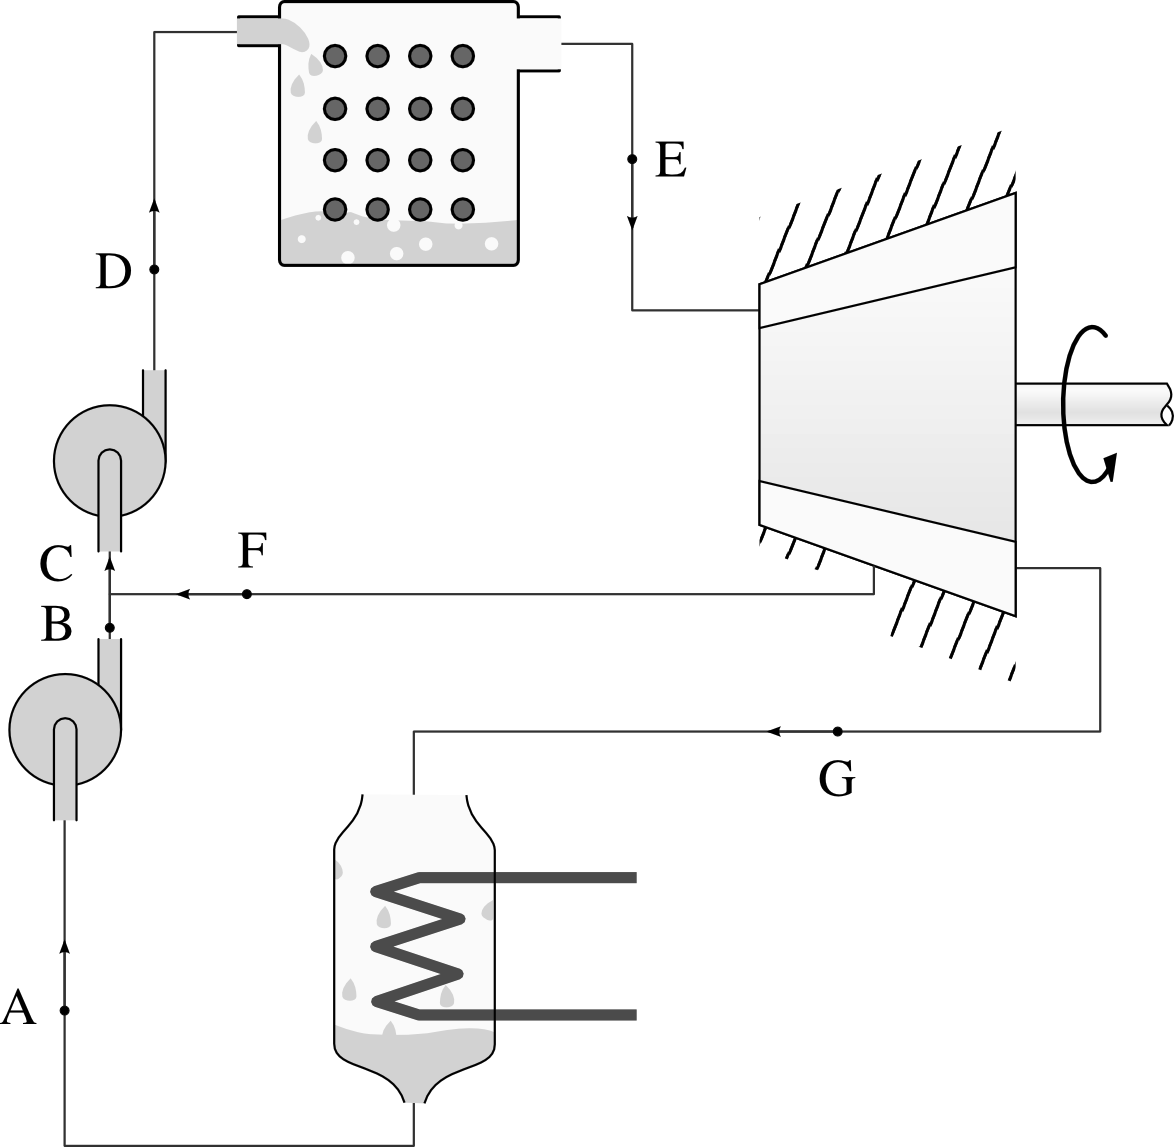
\includegraphics[height=11cm]{images/circuit_prelevement.png}
			\end{center}
			\caption{Circuit d’une centrale à vapeur avec prélèvement de vapeur. La vapeur extraite prématurément de la turbine est utilisée pour réchauffer l’eau liquide pendant le pompage.}
			\label{fig_cycle_prélèvement_vapeur}
		\end{figure}

		\begin{figure}
			\begin{center}
				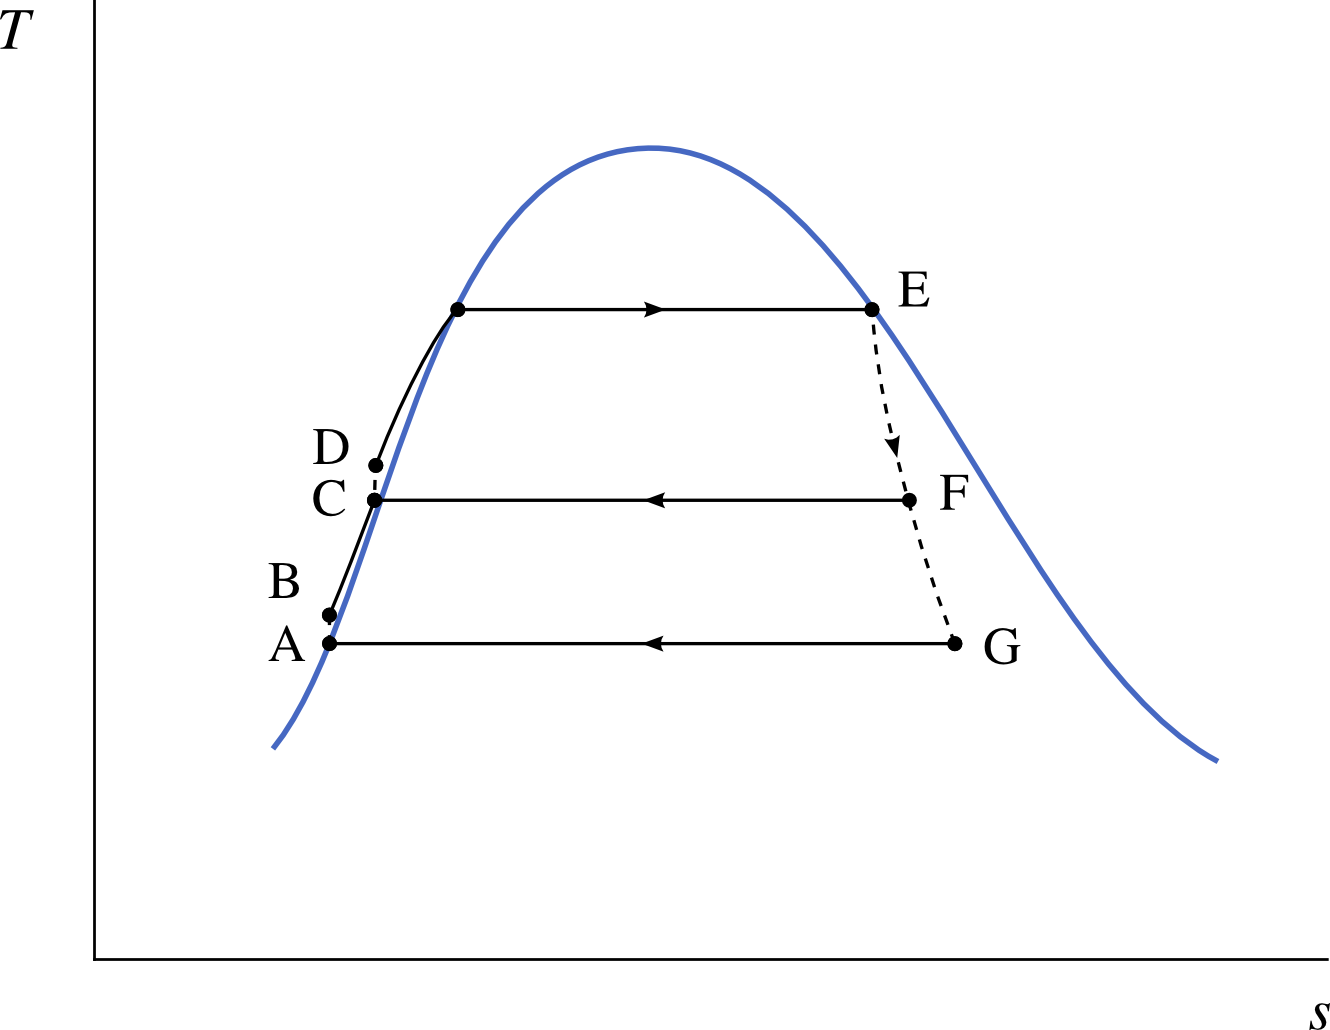
\includegraphics[width=10cm]{images/ts_lv_prelevement.png}
			\end{center}
			\caption{Diagramme température-entropie d’une centrale à vapeur avec prélèvement de vapeur.}
			\label{fig_ts_lv_prelevement_vapeur}
		\end{figure}

		En pratique, de nombreux prélèvements (judicieusement appelés \vocab{bleeds} en anglais) sont effectués dans les circuits de centrale à vapeur, pour contrôler les flux de chaleur (\cref{fig_grosse_centrale_vapeur}). Ils permettent accessoirement, par le biais de vannes de décharge, de réguler précisément les débits de masse et adapter ainsi rapidement la puissance de l’installation à la demande.

		\begin{landscape}
		\begin{figure}
		 	\begin{center}
		 			\vspace{-1cm}
				\centerline{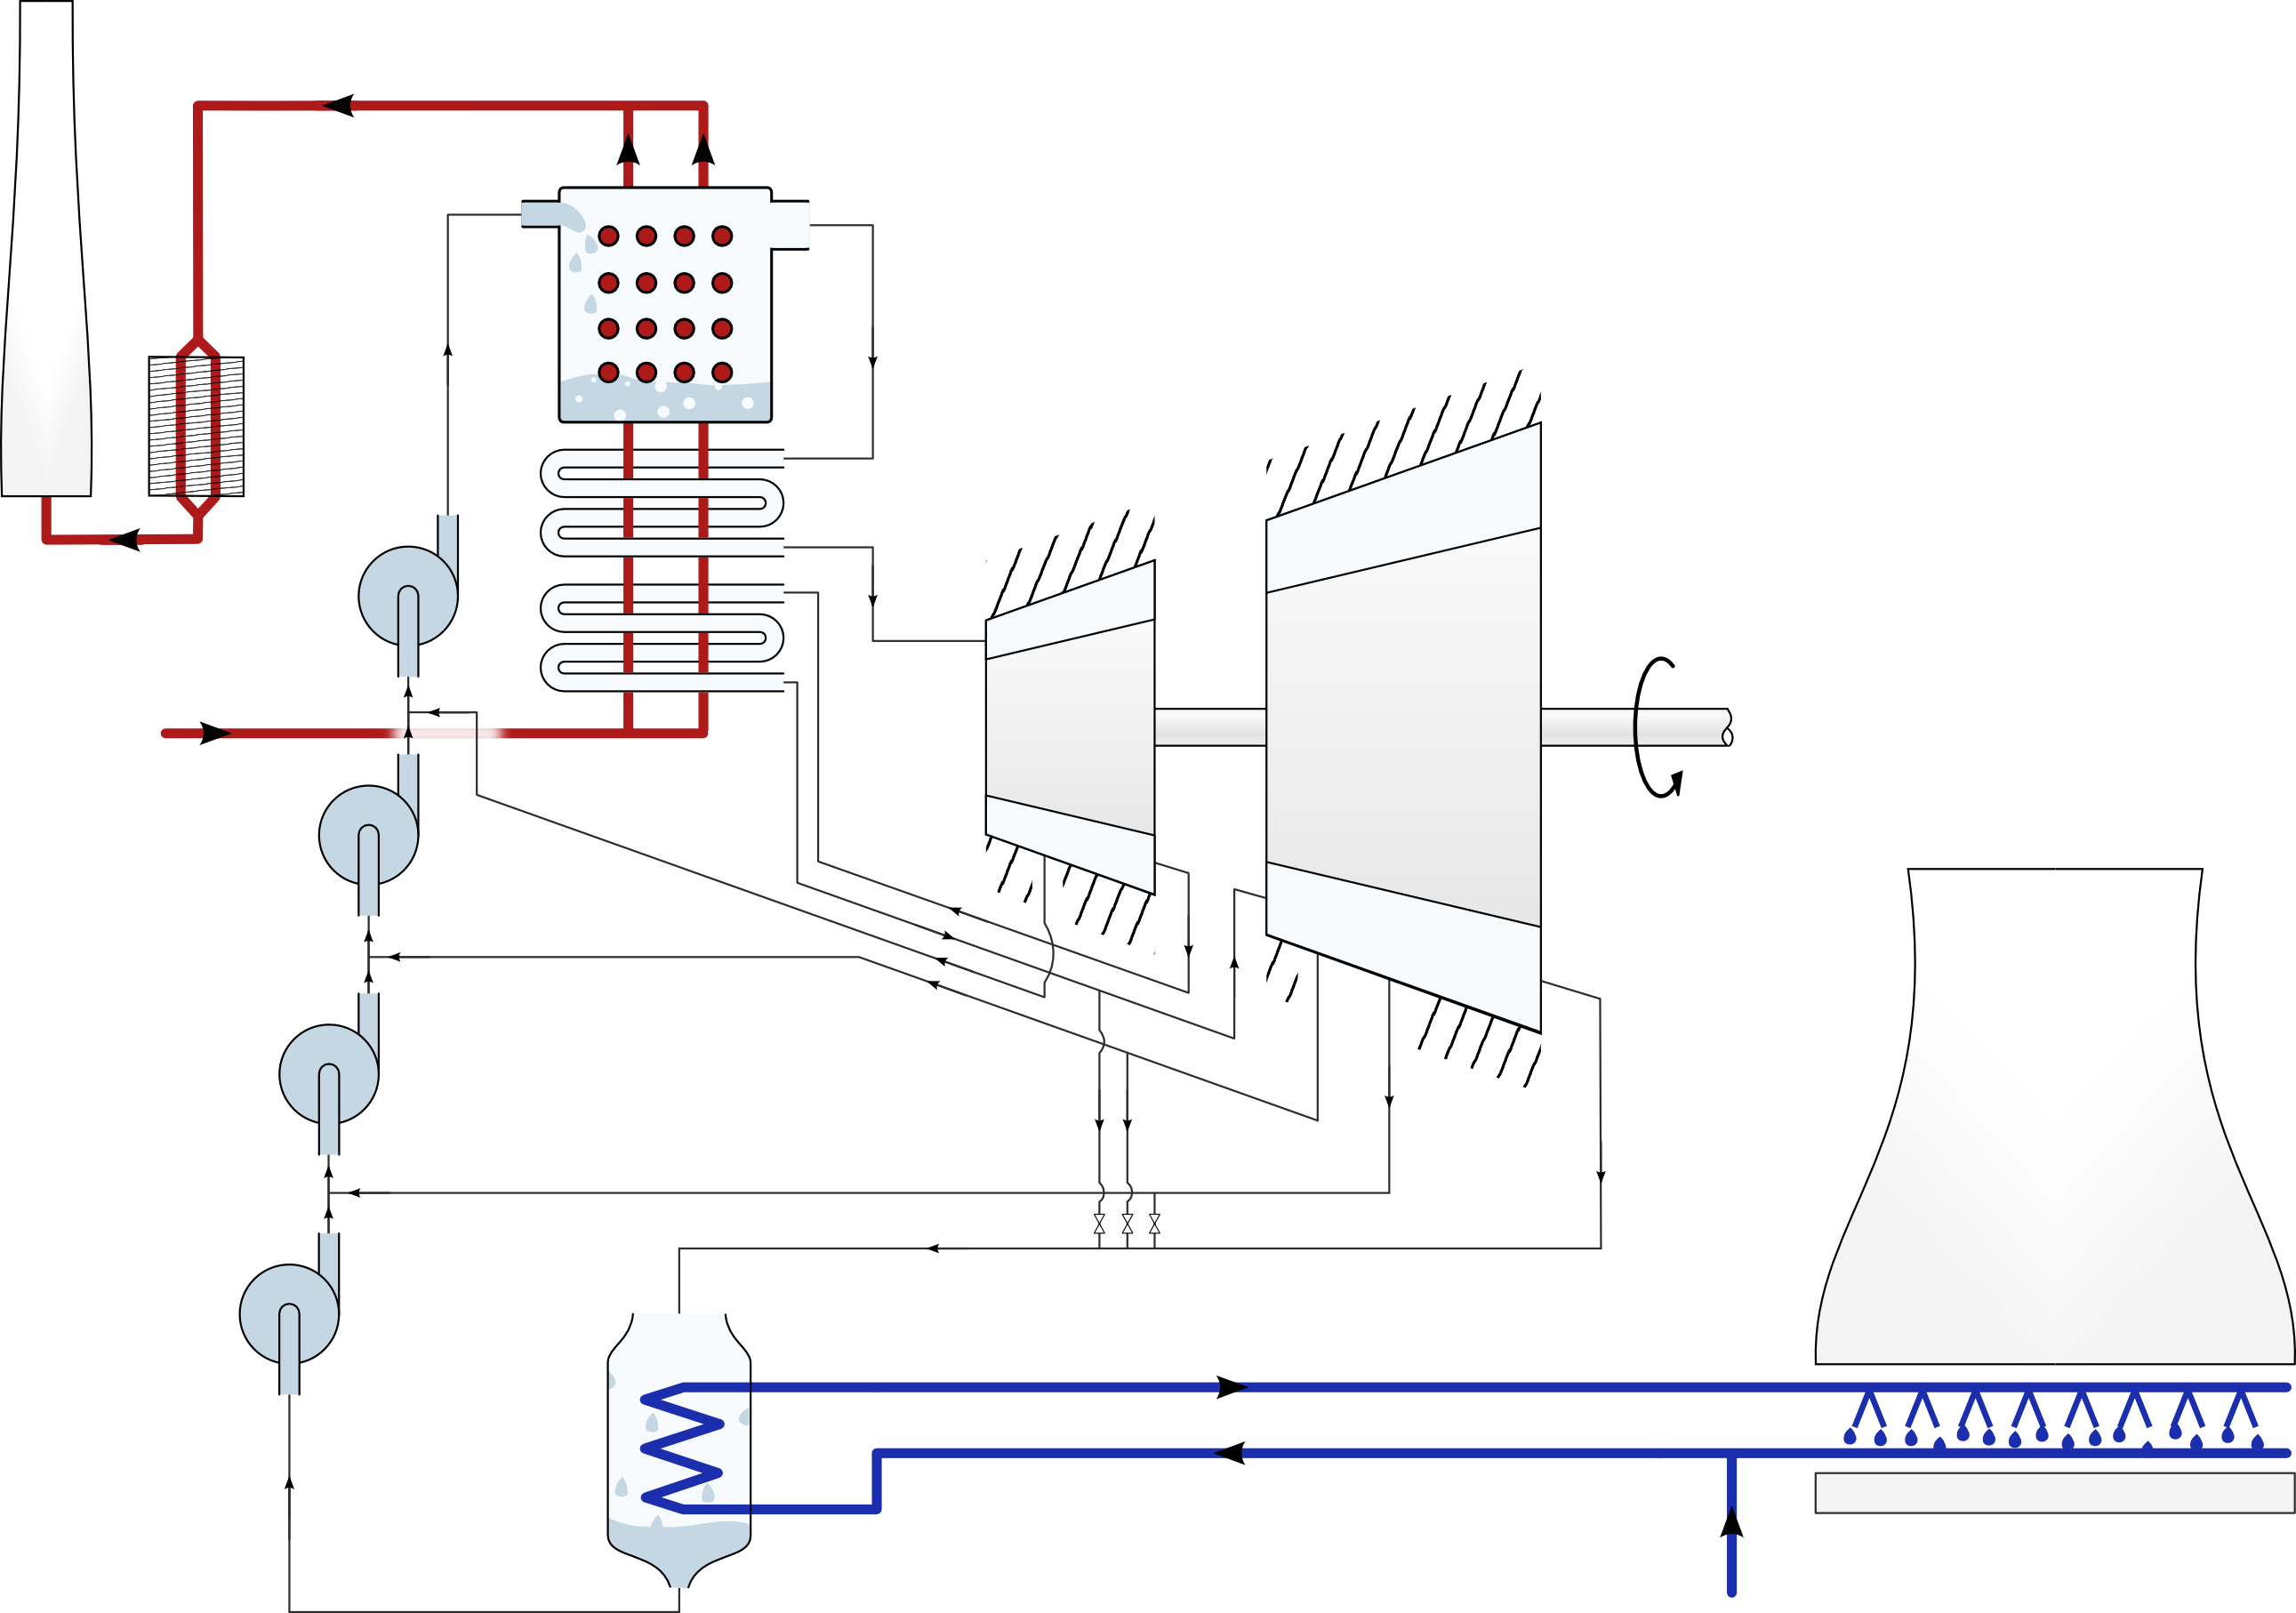
\includegraphics[width=20cm]{images/circuit_complet.png}}
			\end{center}
			\caption{Installation à vapeur mêlant surchauffe, resurchauffe, régénération, et conduits de décharge.
		Il est laissé à l’étudiant/e curieux/se le loisir de tracer les évolutions sur un diagramme température-entropie, et de s’imaginer aux commandes de l’installation alimentant sa cafetière en électricité.}
			\label{fig_grosse_centrale_vapeur}
		\end{figure}
		\end{landscape}

\atstartofhistorysection
\section[Un peu d’histoire : de la turbine à vapeur à la turbine à gaz]{Un peu d’histoire :\onlyamphibook{\\} De la turbine à vapeur\onlyamphibook{\\} à la turbine à gaz}
\label{ch_histoire_turbine}\index{turbine!histoire de la}\index{turbomachine (moteur à turbine)}

\index{Turbinia (navire)}\index{Parsons, Charles Algernon}
Au début du \textsc{xx}\ieme siècle, la \vocab[turbomachine (moteur à turbine)]{turbine} a remplacé les pistons et cylindres dans tous les moteurs à vapeur. 
Une turbine est une pièce de géométrie complexe, sensible aux imperfections de fabrication, ce qui rend sa construction plus délicate que celle de pistons cylindriques. En contrepartie, on obtient un moteur d’agencement simple, vibrant peu, et plus facile à assembler, entretenir et lubrifier, ce qui permet d’augmenter sa puissance ou de réduire son volume. L’ingénieur anglais \wf{Charles Algernon Parsons} le démontre de façon spectaculaire en 1897 avec la \textit{Turbinia} (\cref{fig_turbinia}), premier navire en son genre et si rapide qu’aucun bâtiment militaire ne parvient à le rattraper. Dix ans plus tard, toute la \textit{Royal Navy} est propulsée avec des turbines.

	\onlyframabook{\begin{figure}}
	\onlyamphibook{\begin{figure}[htc]}%handmade
		\begin{center}
			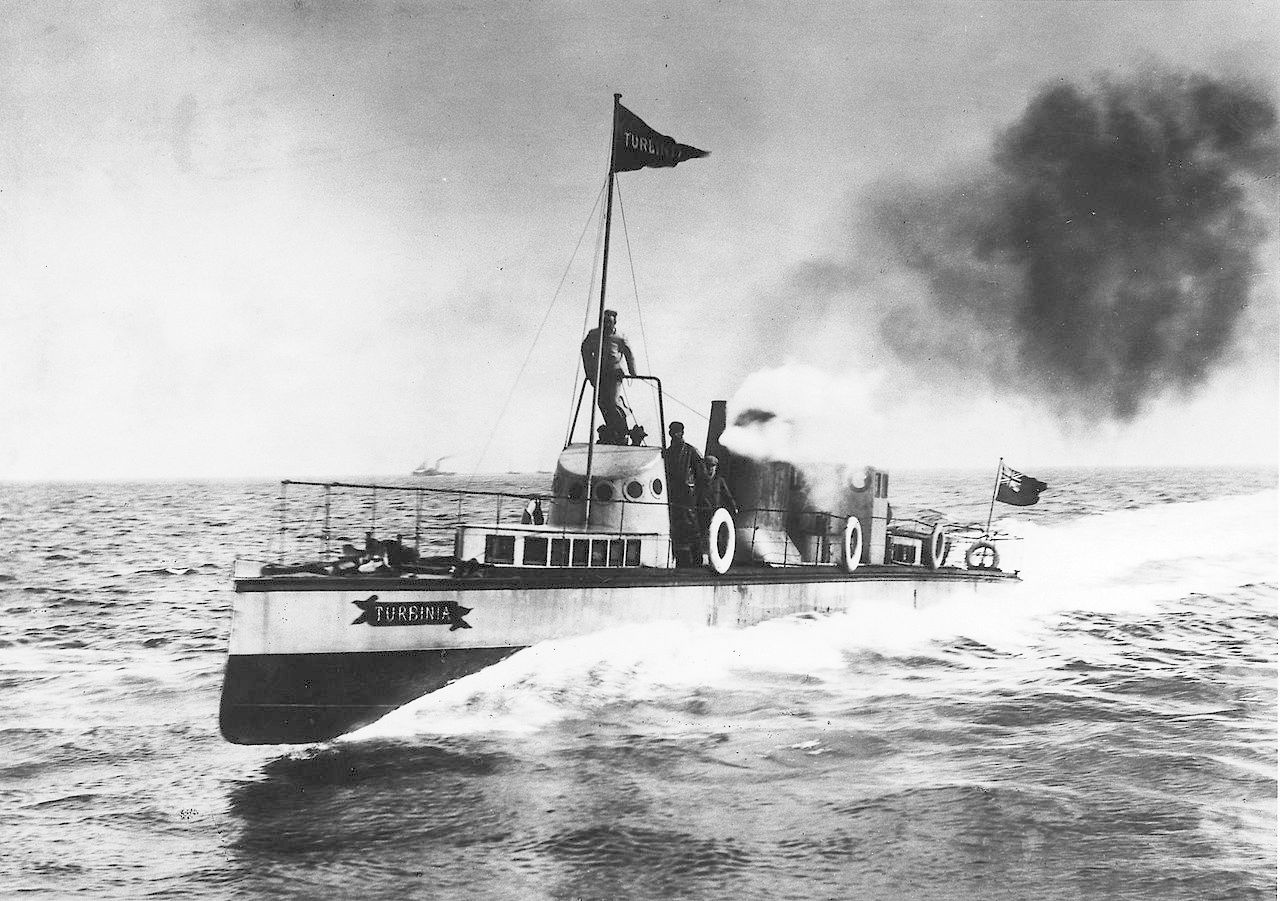
\includegraphics[width=8cm]{images/turbinia.jpg}
			\supercaption{Le \textit{Turbinia}, yatch de Charles Parsons servant de démonstrateur pour ses recherches en propulsion maritime. Avec ses trois turbines à vapeur et ses neuf hélices, il atteint \SI[per-mode=symbol]{60}{\kilo\metre\per\hour} et permet à son propriétaire de ridiculiser la \textit{Royal Navy} pendant le défilé du \textit{Jubilee} de la reine Victoria en 1897.}%
				{\wcfile{Turbinia At Speed.jpg}{photo} par Alfred John West, 1897 (\pd)}
			\label{fig_turbinia}
		\end{center}
	\end{figure}

\index{von Ohain, Hans}\index{Ohain, Hans von}\index{Whittle, Frank}
Dans l’univers des moteurs à gaz, la situation est tout autre : jusqu’à la fin des années 1930, tous les moteurs sont à pistons-cylindres. Cette technologie culmine dans le secteur aéronautique, où l’on arrange les cylindres en étoiles derrière les hélices, pour réduire l’encombrement et les vibrations engendrées. Dans ces machines, telles que le \textit{Twin Wasp} de \textit{Pratt \& Whitney}, l’arrangement mécanique des cylindres, bielles et vilebrequins est absolument phénoménal (\cref{fig_twin_wasp}), et les circuits d’alimentation et de vidange des dizaines de chambres de combustion différentes sont labyrinthiques. Deux ingénieurs, l’allemand \wf{Hans von Ohain} et l’anglais \wf{Frank Whittle}, se consacrent indépendamment à la conception d’un moteur à turbine destiné à s’affranchir de cette complexité.


	\onlyframabook{\begin{figure}}
	\onlyamphibook{\begin{figure}[htc]}%handmade
		\begin{center}
			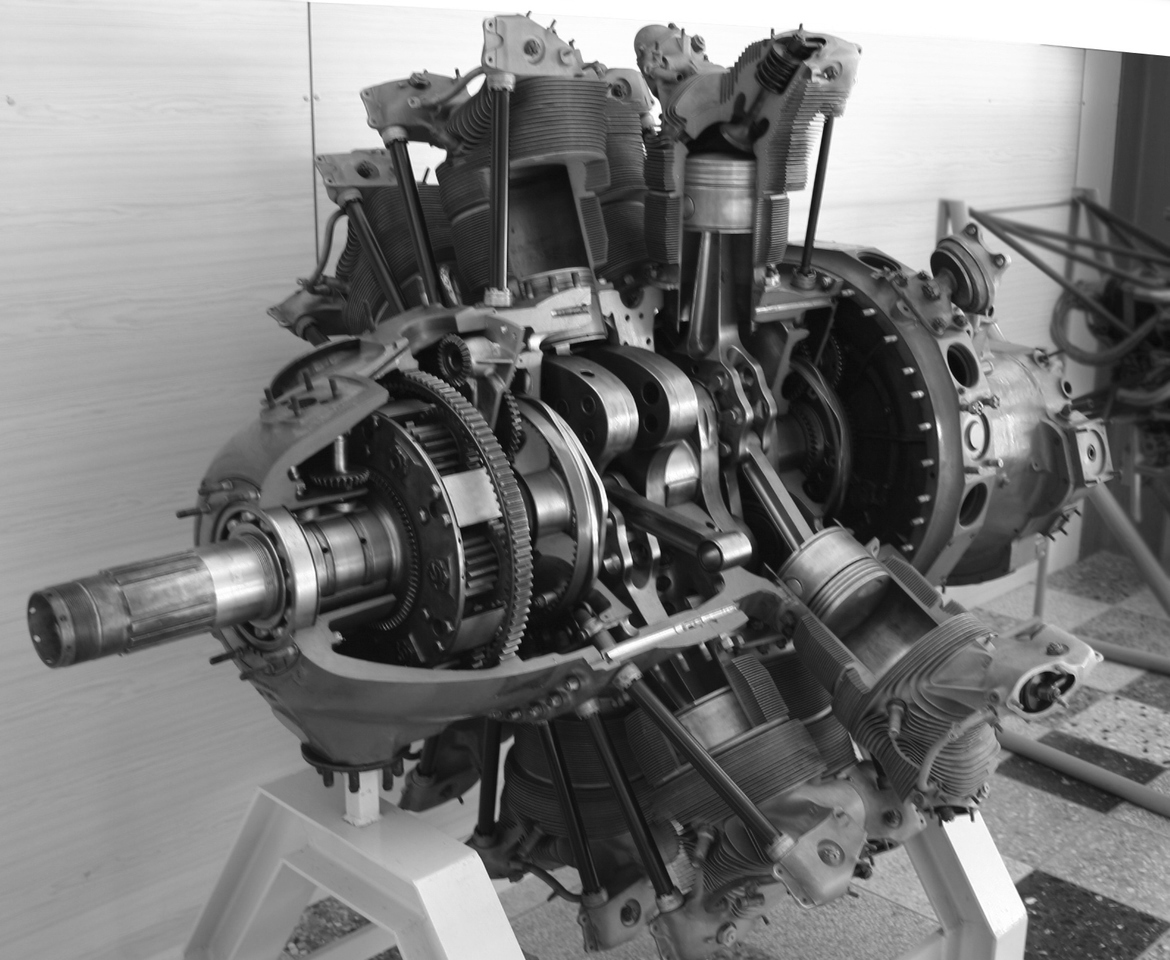
\includegraphics[width=8cm]{images/twin_wasp.jpg}
			\supercaption{Découpe d’un moteur \textit{Pratt \& Whitney Twin Wasp} (1932), montrant l’arrangement intérieur avec bielles et vilebrequins reliant les deux rangées de sept pistons agencés en étoile. Le moteur, de cylindrée \SI{30}{\liter}, dégageait plus de \SI{1000}{ch} et a été produit à plus de \num{170 000} exemplaires.}%
				{photo \ccbysa \olivier}
			\label{fig_twin_wasp}
		\end{center}
	\end{figure}

La mise au point d’un moteur à turbine est bien plus difficile pour les gaz que pour la vapeur. Certes, l’air (ou les gaz brûlés) et la vapeur sèche ont des propriétés très similaires : ainsi une turbine à vapeur fonctionne très bien avec de l’air comprimé. La difficulté se trouve à l’autre extrémité du moteur. Dans les moteurs à vapeur la compression de l’eau est faite à l’état liquide, ce qui est très économe. Compresser de l’eau à \SI{10}{\degreeCelsius} de \num{1} à \SI{10}{\bar}, par exemple, ne requiert que $w_\fromatob \approx v_L (p_\B - p_\A ) = \num{0,001} (10 - 1) \times \num{e5} = \SI{900}{\joule\per\kilogram}$ (\ref{eq_pompe_liquide}). Par contraste, faire de même avec de l’air demande une puissance spécifique minimale de $w_\fromatob = c_p \Delta T = c_p \left( T_\A \left(p_\B/p_\A\right)^\frac{\gamma - 1}{\gamma} - T_\A \right) = \num{1005} \left(\num{283,15} \left(10\right)^\frac{\num{0,4}}{\num{1,4}} - \num{283,15} \right) = \SI{265}{\kilo\joule\per\kilogram}$ (\ref{eq_gp_travail_isentropique_so} \& \ref{eq_isentropique_horrible2}), soit presque trois cents fois plus !

\index{efficacité!isentropique}\index{turbine!efficacité d’une}\index{compresseur!efficacité d’un}\index{efficacité!d’un compresseur}\index{efficacité!d’une turbine}
Nous avons vu en \S\ref{ch_cycle_de_rankine} que la compression liquide n’est pas sans contrepartie – elle doit être compensée par une plus grande puissance à la chaudière et réduit le rendement thermodynamique — mais elle facilite grandement la mise au point du moteur. Comme la quasi-totalité de la puissance nette du moteur provient de la turbine, une détente peu réversible ou incomplète n’affecte «~que~» la puissance et le rendement du moteur. Dans une turbomachine à gaz, en revanche, la turbine alimente aussi le compresseur : elle joue donc un rôle double. Tant qu’elle ne dégage pas une puissance suffisante pour égaler celle du compresseur, le moteur ne fonctionne pas du tout. L’efficacité isentropique de la turbine et du compresseur deviennent de fait des paramètres primordiaux (nous y reviendrons en \S\ref{ch_rapport_des_puissances} avec la notion de \vocab{marge de travail}\index{travail!marge de}) et il s’ensuit que la mise au point de la turbomachine à gaz est une entreprise ambitieuse.

\index{von Ohain, Hans}\index{Ohain, Hans von}\index{Whittle, Frank}\index{fiabilité}\index{moteur!fiabilité d’un}
Whittle et von Ohain vont tous deux concentrer leurs efforts sur un moteur aéronautique ingénieux nommé \vocab{turboréacteur}\index{turboréacteur!à simple flux} : ce sont les gaz d’échappement, en grande quantité et avec une forte pression résiduelle, qui vont fournir la poussée du moteur (\S\ref{ch_turboreacteur}). Le principe de fonctionnement est simplissime (le flux d’air est ininterrompu et il n’y a qu’une pièce mobile) mais les défis sont nombreux. Comme une aile d’avion, les pales du compresseur ont tendance à décrocher à faible puissance et dans les phases transitoires, provoquant des variations de débit brutales et destructrices. Dans les chambres de combustion, il faut empêcher la flamme de lécher les parois (ce qui provoquerait leur fonte) ou de se prolonger, en particulier lors des allumages ou rallumages, dans la turbine. Les contraintes de poids nécessitent l’emploi de matériaux légers qui compliquent la fabrication. Les deux ingénieurs conduisent leurs travaux en plein cœur de la seconde guerre mondiale, chacun financé par des budgets militaires, et les premiers avions à réaction volent en 1940. Les appareils de série qui suivent sont délicats d’utilisation, peu réactifs et leur durée de vie en service atteint à peine \SI{20}{\hour}. Ils arriveront trop tard et en nombre trop faible pour affecter le cours du conflit.

	\begin{figure}
		\begin{center}
			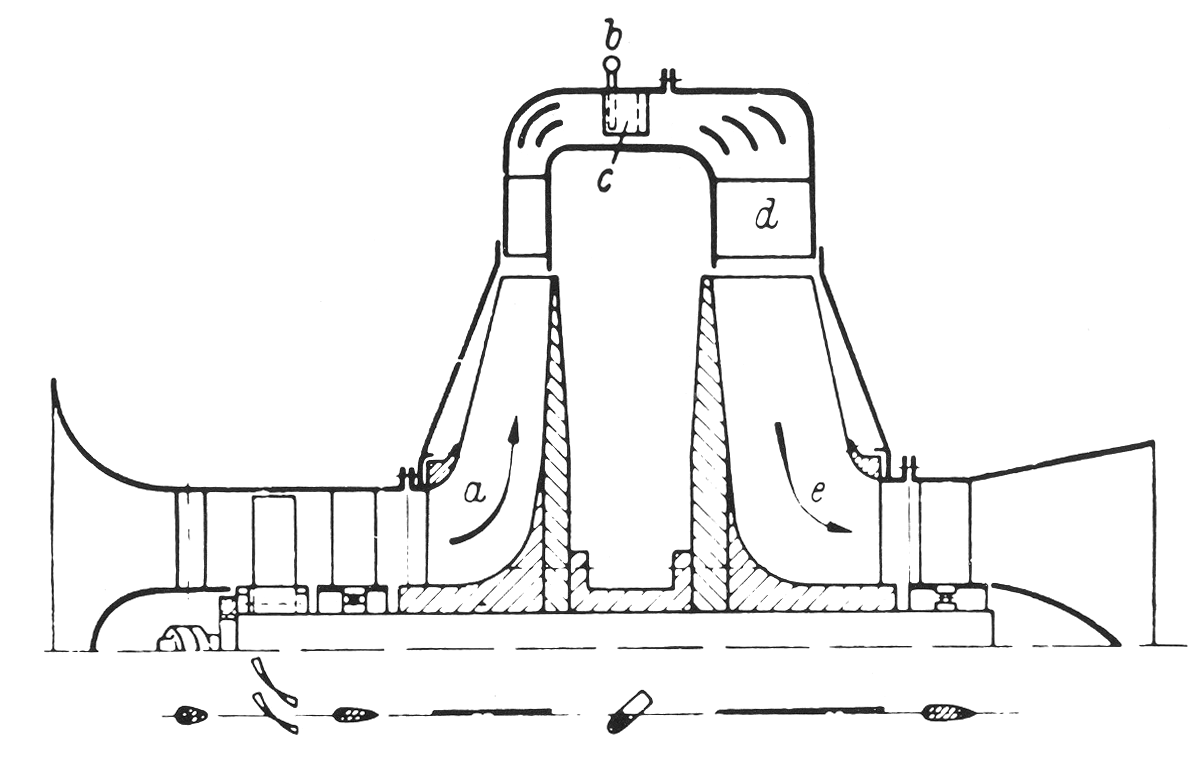
\includegraphics[width=8cm]{images/he_s1.png}
			\supercaption{Schéma de coupe du \textit{Heinkel He S-1}, premier prototype testé par Hans von Ohain en 1937. Le compresseur est constitué d’un étage axial et d’un étage centrifuge ; la turbine est centripète. Il n’y a qu’une pièce mobile et sa vitesse est uniforme.\index{compresseur!centrifuge}}%
				{\wcfile{Ohain USAF He S-1 page58.jpg}{schéma} USAF (\pd)}
			\label{fig_turbinia}
		\end{center}
	\end{figure}

À la fin de la guerre, c’est l’engouement : l’aviation s’empare du moteur qu’elle attendait depuis trois décennies. Pour comprendre ce qui fait du turboréacteur le Graal de l’aéronautique du \textsc{xx}\ieme siècle, il faut un peu de mécanique du vol. En vol subsonique, un appareil correctement dessiné a un \vocab{coefficient de traînée}\index{traînée, coefficient de} $C_x \equiv F_x \div \left(\frac{1}{2} S_\text{réf.} \rho \ C_\text{vol}^2\right)$ quasi-constant. Ainsi, lorsque l’on réduit la surface alaire $S_\text{réf.}$ et la masse volumique ambiante $\rho$ (en gagnant de l’altitude), on peut augmenter la vitesse de vol $C_\text{vol}$ \emph{en maintenant la traînée $F_x$ constante}. Le coût énergétique du déplacement de l’avion reste alors constant -- en revanche, la puissance à fournir $\dot W_\text{moteur} = F_x C_\text{vol}$, elle, augmente proportionnellement à la vitesse. Ces caractéristiques font des avions des machines relativement économes en énergie, mais très gourmandes en puissance, puisqu’il leur faut maintenir la même poussée à très haute vitesse.

\index{poussée!spécifique}\index{spécifique!poussée}\index{puissance!spécifique (d’un moteur)}\index{spécifique!puissance}
Le turboréacteur a deux atouts pour répondre à ce problème. D’une part, il est compact, léger et sans vibration, ce qui est très désirable pour une application où la traînée (et donc la poussée à fournir) augmente proportionnellement au poids de la machine. D’autre part l’hélice, très efficace en vol lent mais dont les embouts de pale arrivent tôt à des vitesses supersoniques et limitent de ce fait la vitesse des avions, est purement supprimée. Ces deux qualités rendent acceptables les faibles efficacités dues aux compressions et détentes peu réversibles, aux faibles taux de pression et aux vitesses exagérément hautes atteintes par les gaz dans les tuyères.

Ainsi, le gracieux \textit{Lockheed Constellation}, culmination de l’ère de l’aviation à hélice, est rendu instantanément obsolète par l’arrivée en 1949 du \textit{De Havilland Comet}, prodigieux quadriréacteur de même taille mais beaucoup plus rapide (\cref{fig_trois_avions}). Même s’il ne peut initialement franchir la même distance et que sa consommation kilométrique de carburant est plus haute, le \textit{Comet} ne laisse aucune chance à ses concurrents. Sa rapidité est une qualité évidente pour les passagers, mais aussi pour les compagnies dont il augmente nettement la productivité.

	\begin{figure}[htc]
		\begin{center}
			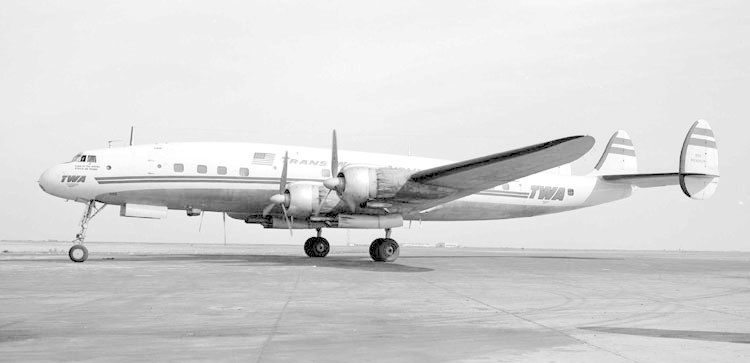
\includegraphics[width=9cm]{images/lockheed_constellation.jpg}
			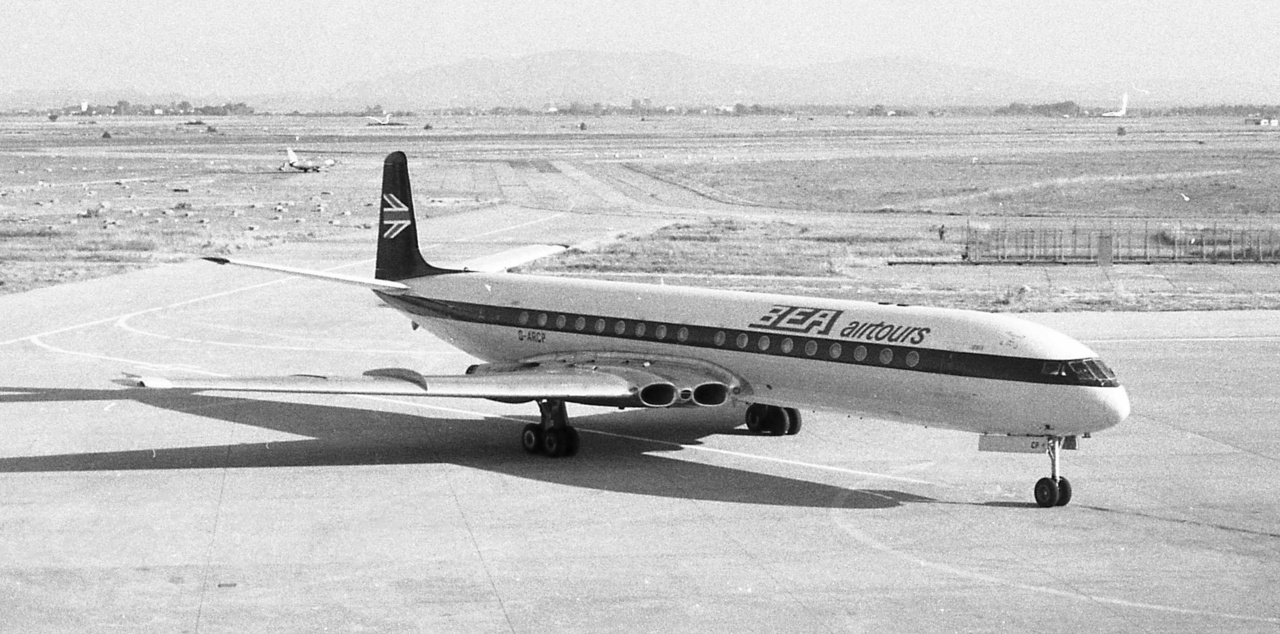
\includegraphics[width=9cm]{images/dhc_comet.jpg}
			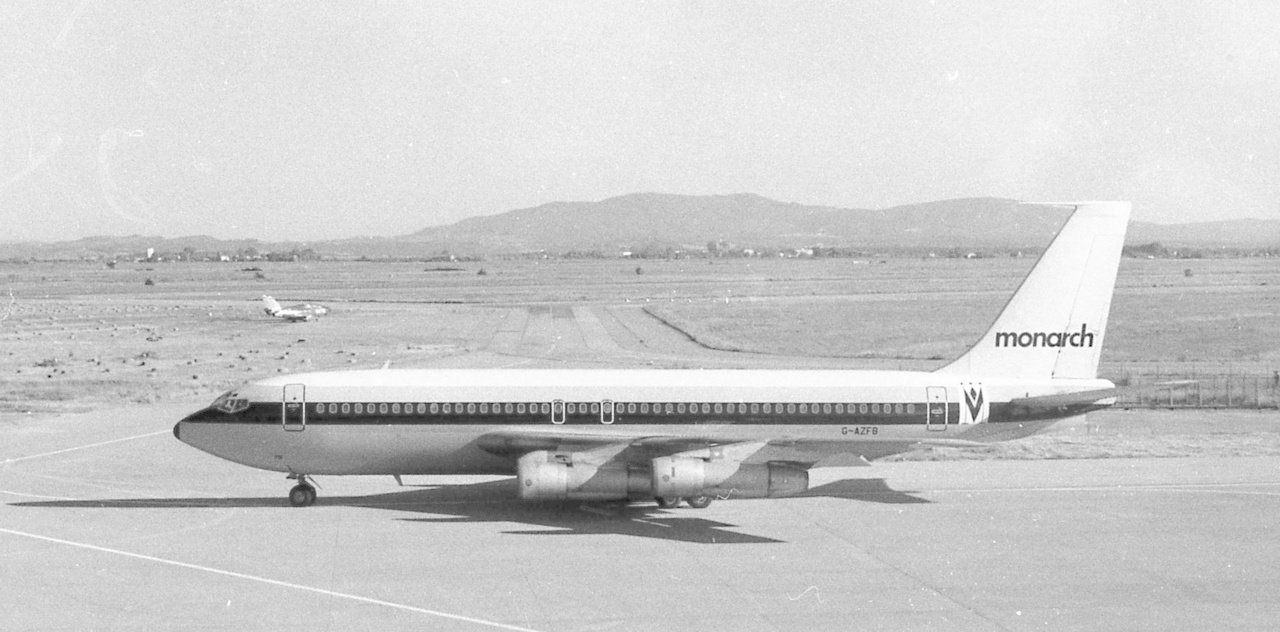
\includegraphics[width=9cm]{images/boeing_707.jpg}
			\supercaption{De haut en bas:\\%
				Le \textit{Lockheed Constellation} (1943), aboutissement de l’ère de l’aviation à hélice : quatre moteurs \textit{Wright Duplex-Cyclone} surcompressés à 18 cylindres chacun, capable de franchir \SI{3700}{\kilo\metre} à \SI[per-mode=symbol]{500}{\kilo\metre\per\hour}.\\%
				Le \textit{De Havilland Comet} (1949), premier avion de ligne à réaction : quatre turboréacteurs \textit{Halford Ghost} monoflux, capable de franchir \SI{2400}{\kilo\metre} à \SI[per-mode=symbol]{740}{\kilo\metre\per\hour}.\\%
				Le \textit{Boeing 707} (1957), dont la configuration et les performances préfigurent celles de tous ses successeurs depuis : quatre turboréacteurs \textit{Pratt \& Whitney JT3C} monoflux, capable de franchir \SI{4300}{\kilo\metre} à \SI[per-mode=symbol]{900}{\kilo\metre\per\hour}.}%
				{\wcfile{Lockheed1049twa (4423687925).jpg}{photo Constellation} \ccbysa par Bill Larkins\\%
				 \wcfile{BEA Airtours Comet G-ARCP 1N.jpg}{photo Comet} et \wcfile{Monarch B-720 G-AZFB 4N.jpg}{707} (retouchées) \ccbysa par Piergiuliano Chesi}
			\label{fig_trois_avions}
		\end{center}
	\end{figure}


Le \textit{Comet}, après la rectification d’un grave défaut de conception, sera lui-même rattrapé par le \textit{Boeing 707} en 1957. Capable de voler plus loin en emportant plus, et encore plus rapide (à \SI[per-mode=symbol]{900}{\kilo\metre\per\hour}, la vitesse que tous les avions de ligne ont adopté depuis, l’air à l’extrados des ailes atteint tout juste la vitesse du son), le \textit{707} marque l’entrée dans l’\textit{ère du jet}, dans laquelle les avions de ligne ne se fabriquent plus par dizaines mais par milliers. Ainsi en vingt-cinq années seulement la turbomachine à gaz a doublé la vitesse des avions et divisé par quatre le prix des billets.
%\onlyamphibook{\pagebreak}%handmade bien pourri, vraiment honteux


%\onlyamphibook{\clearfloats}%handmade
%handmade quote (sur 2 colonnes dans l’amphibook, {quote} est trop étroit
	\onlyframabook{\begin{quote}}
	\onlyamphibook{\begin{historyquote}}
	\begin{footnotesize}
		«~Parés ?~» «~Décollage, top !~» Le mécano pousse avec moi sur les manettes.\\
		NNggnniiiaavvrrooooooaaaaaaarrrrooouuummmmm…\\
		«~N1 vert~». Ça pousse sévère, mais ça accélère tout doucement, étant donné le poids du mastodonte.\\
		«~80 nœuds~» «~Poussée disponible~»\\
		J’ai le bout des pieds sur le palonnier, une précision de tatane similaire à un avion à train classique. Je me régale.\\
		120 nœuds. Au palonnier, je maîtrise, les mecs. 432 passagers et 15 navigants sont accrochés derrière, l’oreille et les sens aux aguets.\\
		140 nœuds. Deux rafales de balises lumineuses défilent sur les côtés. Le palonnier, pointu.
		
		«~V1~» Encore 20 nœuds à prendre pour que l'engin puisse voler. Voilà le bout qui arrive, là-bas devant.\\
		«~Rotation~». À 170 nœuds, je tire doucement, puis plus fermement.\\
		Cinq degrés d'assiette. Dix degrés. Ça s’arrête de rouler, l’aiguille est à 185~nœuds.\\
		Assiette douze degrés. Hue, Cocotte, il faut monter.\\
		«~Vario positif~» «~Train sur rentré~». La vérité se situe ce soir entre douze et treize degrés d’assiette, c'est là que l'aiguille du badin s'immobilise. On passe la côte, et trois-cent pieds en dessous, le passage du \textit{747} doit tenir du séisme.
			\begin{flushright}\vspace{-0.5em}Jacques Darolles, 1998\\ \textit{Le plus beau bureau du monde}~\cite{darolles2000}\end{flushright}\index{Darolles, Jacques}
	\end{footnotesize}
	\onlyamphibook{\end{historyquote}}
	\onlyframabook{\end{quote}}

\index{fiabilité}\index{moteur!fiabilité d’un}
Presque soixante ans après le premier vol du \textit{707}, les avions de ligne volent toujours à la même vitesse, mais la technologie des turboréacteurs n’a cessé de progresser~\cite{rollsroyce2005}. Avec leurs pales de soufflante en composite carbone-époxy ou en titane soufflé, stators de turbine imprimés en céramique, multiples circuits pneumatiques de refroidissement de turbine percés au laser, leurs systèmes électroniques de contrôle, de diagnostic et de surveillance par télétransmission, ils continuent lentement d’augmenter en efficacité. La fiabilité n’est pas en reste : un moteur moderne ne subit en moyenne qu’une défaillance en vol toutes les \num{200 000} heures de vol, et n’est séparé de l’avion pour maintenance que toutes les \num{20 000} heures ou \num{10 000} vols. Un nouveau type de moteur pourra-t-il jamais rendre le turboréacteur obsolète et propulser de nouveau l’aviation vers une nouvelle~ère ?

\atendofhistorysection


\atstartofexercices
	\begin{boiboiboite}
	\propeau
	\propair
\end{boiboiboite}

\subsubsection{Cycle de Rankine}
	\label{exo_porcheville_rankine}

\begin{comment}
	1.800 tonnes/heure
	Fioul 10×plus cher que le charbon (1000 euros/tonne vs 100 euros)
	Chaque chaudière, 545° 180 bar, 130t fioul/heure
	Pression entrante turbines 150 bars
	Température de l’eau vers la seine: 3°C
	
	Charbon environ 35 MJ/kg
	
\end{comment}

	La centrale EDF de Porcheville (\cref{fig_porcheville}), en bordure de l’A13 à Mantes-la-Jolie, reçoit de la chaleur issue de la combustion de fioul, et utilise un cycle à vapeur pour alimenter une génératrice électrique.
	
	\begin{figure}
		\begin{center}
			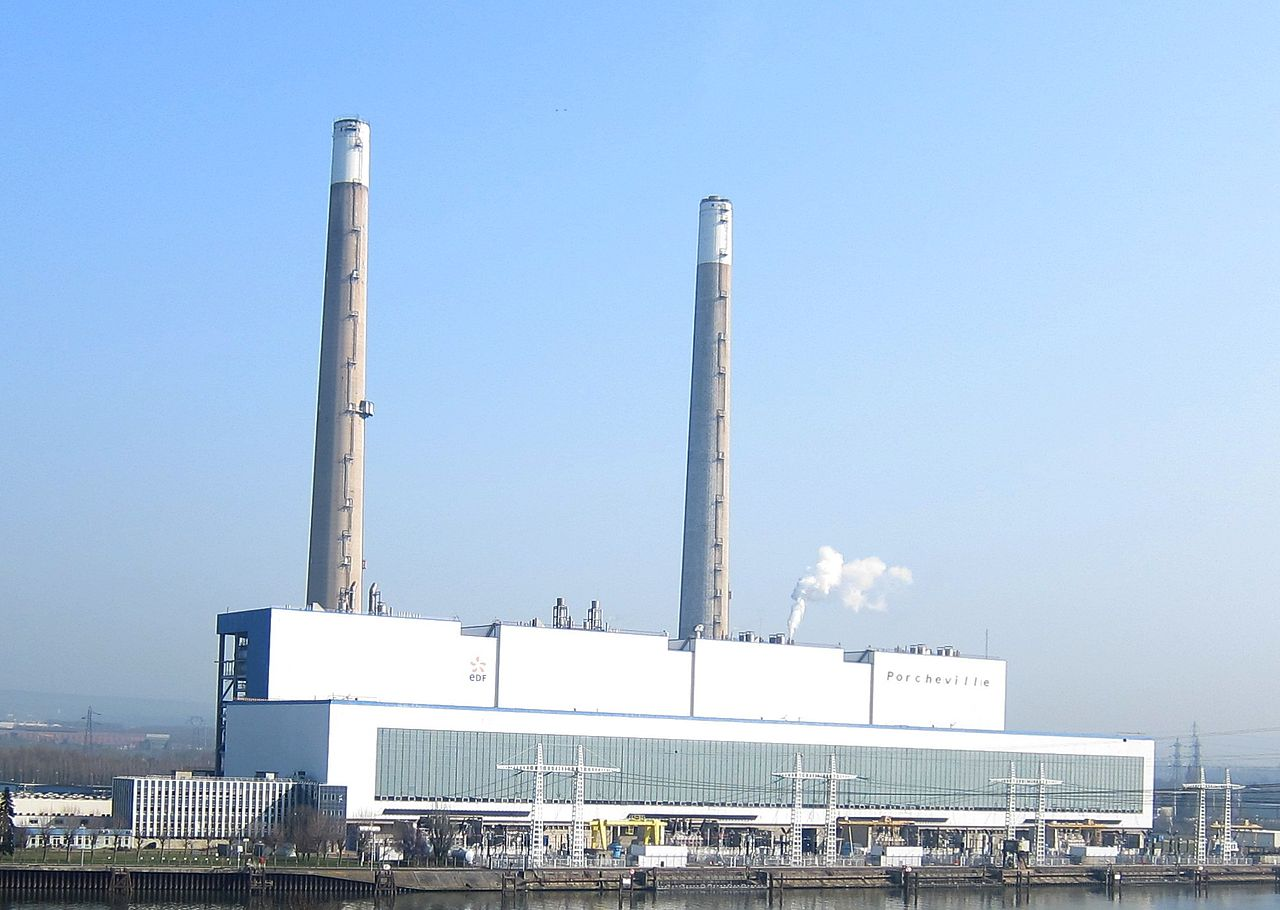
\includegraphics[width=8cm]{images/porcheville.jpg}
			\vspace{-0.5cm}
		\end{center}
		\supercaption{Centrale électrique de Porcheville, alimentée au charbon jusqu’en 1987 et fonctionnant désormais au fioul. Elle sert principalement les demandes de pointe.}{Photo schéma \cczero \oc}
		\label{fig_porcheville}
	\end{figure}
	
	Dans la centrale l’eau évolue entre les pressions de~\SI{0,1}{\bar} et~\SI{140}{\bar}. La vapeur atteint~\SI{545}{\degreeCelsius}, et les turbines ont une efficacité isentropique de~\SI{80}{\percent}.

	Dans cet exercice, nous considérons que le cycle est basé sur un cycle de Rankine surchauffé.
	
	\begin{enumerate}
		\item Schématisez le circuit physique de l’eau dans la centrale ; tracez le cycle suivi sur un diagramme température-entropie.
		\item Quelle est l’enthalpie spécifique de l’eau à la sortie de la turbine ?
		\item Quelle est l’enthalpie spécifique de l’eau à la sortie des pompes ?
		\item	Quel est le rendement thermodynamique de l’installation ?
		\item Quelle est la consommation spécifique de l’installation, c’est-à-dire la masse de vapeur ayant traversé la turbine lorsque l’installation a généré \SI{1}{\kWh} d’énergie mécanique ?
		\item Quel débit horaire de vapeur faut-il faire circuler dans le circuit pour obtenir une puissance mécanique de~\SI{60}{\mega\watt} ?
	\end{enumerate}
	

\subsubsection{Chaudière de centrale à vapeur}

	Dans une centrale à vapeur, la chaudière fonctionne avec la combustion de bois dans de l’air prélevé dans l’atmosphère. Les briquettes utilisées pour la combustion sont faites de résidus de bois et de biomasse (\cref{fig_sciure}) ; elles ont une capacité calorifique massique de~\SI{15}{\mega\joule\per\kilogram}.
	
	\begin{figure}
		\begin{center}
			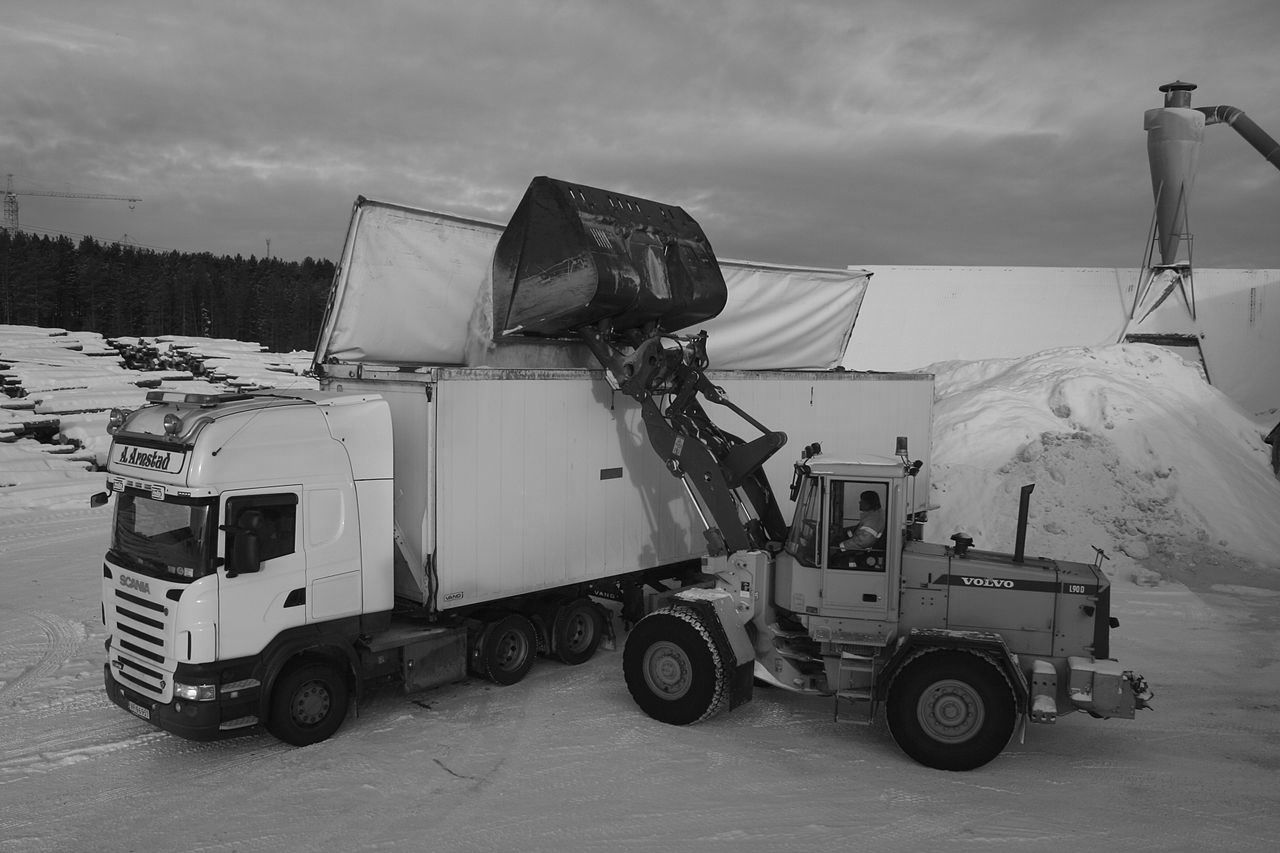
\includegraphics[width=8cm]{images/sciure.jpg}
		\end{center}
		\supercaption{La sciure de bois, produite en très grande quantité dans l’industrie, peut être utilisée comme source d’énergie dans une centrale à vapeur.}{\wcfile{Flislasting.jpg}{Photo} \ccbysa par \wcu{Eivindmy}}
		\label{fig_sciure}
	\end{figure}
	
	L’air pénètre dans la chaudière à température de~\SI{15}{\degreeCelsius} et pression de~\SI{1}{\bar}. Il est porté à température de~\SI{1000}{\degreeCelsius} par combustion à pression constante, avant de passer autour des conduits d’eau.	Lorsqu’il quitte la chaudière, sa température est de~\SI{180}{\degreeCelsius}.

	L’eau pénètre dans la chaudière à~\SI{50}{\bar} et~\SI{20}{\degreeCelsius}. Elle y circule à pression constante. On souhaite la porter jusqu’à une température de~\SI{850}{\degreeCelsius}, avec un débit de~\SI{3}{\kilogram\per\second}.
	
	\begin{enumerate}
		\item Quel débit d’air faut-il admettre dans la chaudière pour respecter le cahier des charges ?
		\item Quelle est l’efficacité de la chaudière ?
		\item Un/e ingénieur/e propose de faire passer le conduit d’air d’admission au travers des gaz d’échappement (sans pourtant les mélanger) pour augmenter la température de l’air avant combustion. Cela vous paraît-il être une bonne idée ?
	\end{enumerate}


\subsubsection{Cycle avec resurchauffe}

	L’installation de Porcheville décrite dans l’exercice~\ref{exo_porcheville_rankine} est modifiée pour accueillir une série de tubes de resurchauffe. La détente de l’eau est interrompue à~\SI{18}{\bar} dans la turbine, et la vapeur est ramenée à la température maximale du cycle (c’est-à-dire \SI{545}{\degreeCelsius}).
	
	La centrale est alimentée au fioul lourd dit «~TBTS~», de masse volumique \SI{1050}{\kilogram\per\metre\cubed} et de pouvoir calorifique \SI{40,2}{\mega\joule\per\kilogram}. La chaudière a une efficacité de~\SI{80}{\percent}.
	
	\begin{enumerate}
		\item Quel est le nouveau rendement de l’installation ?
		\item Quelle est la nouvelle consommation spécifique ?
		\item Quel est le débit volumique horaire de carburant nécessaire pour générer \SI{60}{\mega\watt} électriques ?
	\end{enumerate}
	

\subsubsection{Cycle avec régénération}

	Dans un navire brise-glace polaire (\cref{fig_50letpodeby}), une installation à vapeur alimente les hélices à partir d’un réacteur nucléaire.

	\begin{figure}
		\begin{center}
			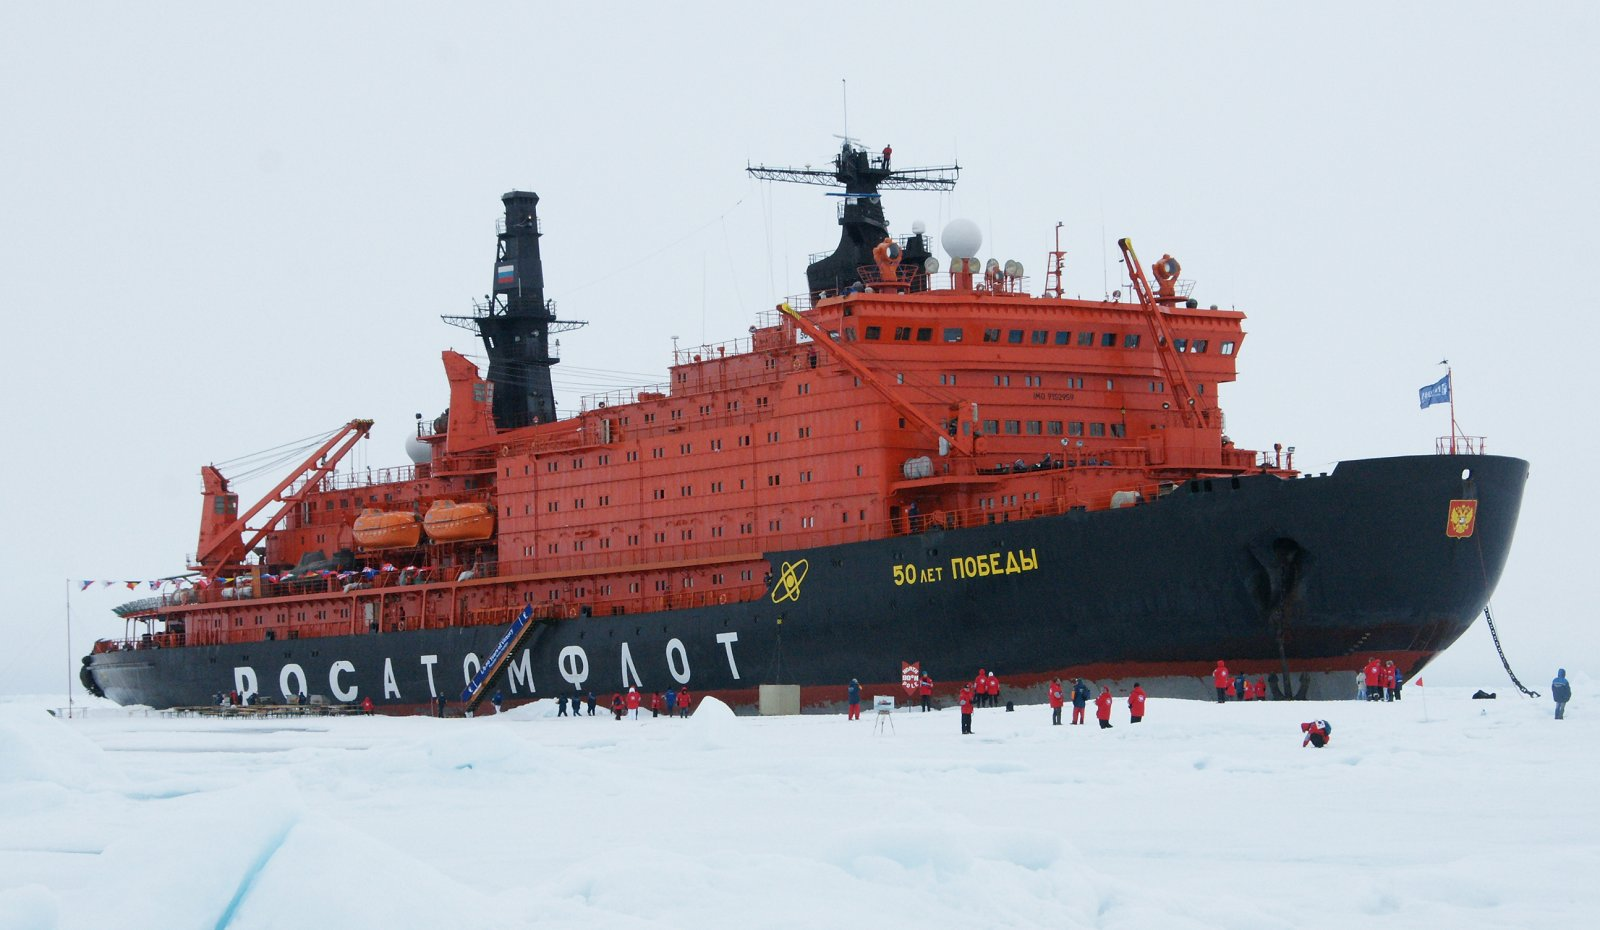
\includegraphics[width=11cm]{images/50letpodeby.jpg}
		\end{center}
		\supercaption{Le 50 Let Podeby, brise-glace de~\SI{25 000}{\tonne} à propulsion nucléo-turbo-électrique (deux réacteurs de~$\SI{171}{\mega\watt}_{\text{chaleur}}$, trois moteurs de~$\SI{17,6}{\mega\watt}_{\text{méch.}}$). Sa construction a débuté en 1989 mais il n’est entré en service qu’en 2007.}{\wcfile{50letPob_pole.JPG}{Photo} \ccbysa par \wcu{Kiselev d}}
		\label{fig_50letpodeby}
	\end{figure}

	Le cycle est basé sur un cycle de Rankine surchauffé à~\SI{310}{\degreeCelsius} (par contact avec les conduites d’eau pressurisée qui, elle, traverse le réacteur), entre les pressions de~\num{30} et~\SI{0,5}{\bar}\footnote{En réalité, entre \num{29} et~\SI{0,75}{\bar}, valeurs qui ne sont pas tabulées dans nos abaques.}. Nous considérons que la turbine est parfaitement isolée et isentropique.% en réalité, 29 et 0,75 bar

	\begin{enumerate}
		\item Quel est le rendement thermodynamique de l’installation ?
		\item On définit la consommation spécifique de vapeur comme l’inverse de la puissance nette de l’installation. C’est la masse de vapeur ayant traversé la turbine lorsque l’installation a généré \SI{1}{\kWh} d’énergie mécanique.\\
			Quelle est la consommation spécifique de l’installation ?
	\end{enumerate}

	Un/e ingénieur/e propose de modifier le cycle pour le rendre régénératif, en prélevant de la vapeur de la turbine pour l’insérer dans le circuit de compression.
	
	Il/elle propose de séparer la compression en deux étapes, l’une de~\num{0,5} à~\SI{6}{\bar}, et la seconde de~\num{6} à~\SI{30}{\bar} ; et d’insérer la vapeur prélevée entre les deux pompes. Le débit de vapeur prélevé est tel que l’eau à la sortie du mélangeur est exactement à saturation.
	
	Pour alléger nos calculs, nous considérons que la puissance de pompage n’est pas modifiée par la régénération.
	
	\begin{enumerate}	
		\shift{2}
		\item Schématisez l’installation proposée (c’est-à-dire le circuit physique suivi par la vapeur).
		\item Représentez le cycle thermodynamique sur un diagramme température-entropie, en traçant la courbe de saturation de l’eau.
		\item Quelle proportion du débit de vapeur faudrait-il prélever à~\SI{6}{\bar} dans la turbine, pour chauffer l’eau à saturation entre les deux pompes ?
		\item La puissance aux hélices augmente-t-elle ou diminue-t-elle, et de combien ?
		\item Le rendement de l’installation augmente-t-il ou diminue-t-il, et de combien ?
	\end{enumerate}

\exercisesolutionpage
\subsubsection*{Résultats}
	\linktosolutionsblurb
	
	\begin{description}
		\item [9.1] \tab 2) $h_\D = \SI{2287,7}{\kilo\joule\per\kilogram} $ 
						\tab 3) $h_\B = \SI{205,9}{\kilo\joule\per\kilogram} $ 
						\tab 4) $\eta_\text{inst.} = \SI{35,29}{\percent}$ 
						\tab 5) $SSC = \SI[per-mode = symbol]{3,15}{\kilogram\per\kilo\watt\per\hour}$ 
						\tab 6) $\dot{m}_\text{eau} = \SI{52,5}{\kilogram\per\second}$
		\item [9.2] \tab 1) $\dot{m}_\text{air} = \SI{15,2}{\kilogram\per\second}$ 
						\tab 2) $\eta_\text{chaud.} = \SI{83,25}{\percent}$
		\item [9.3] \tab 1) $h_{D2} = \SI{2960,8}{\kilo\joule\per\kilogram}$, $h_{E2} = \SI{3570,3}{\kilo\joule\per\kilogram}$, $h_{F} = \SI{2642,7}{\kilo\joule\per\kilogram}$ : $\eta_\text{inst.2} = \SI{36,31}{\percent}$ (\SI{+1}{pt})
						\tab 2) $\dot{V}_\text{carb.} = \SI{17,6}{\metre\cubed\per\hour}$.
		\item [9.4] \tab 1) $h_{A} = \SI{340,5}{\kilo\joule\per\kilogram}$, $h_{B} = \SI{343,54}{\kilo\joule\per\kilogram}$, $h_{C} = \SI{3017,4}{\kilo\joule\per\kilogram}$, $h_{D} = \SI{2284,5}{\kilo\joule\per\kilogram}$ : $\eta_\text{inst.} = \SI{27,294}{\percent}$. 
						\tab 2) $SSC = \SI[per-mode = symbol]{4,93}{\kilogram\per\kilo\watt\per\hour}$ 
						\tab 5) $h_\text{prélèvement} = \SI{2673,9}{\kilo\joule\per\kilogram}$, $h_\text{pré-mélange} = \SI{341,1}{\kilo\joule\per\kilogram}$, $h_\text{post-mélange} = \SI{670,4}{\kilo\joule\per\kilogram}$ : $z = \SI{14,1}{\percent}$
						\tab 6) $w_\text{net~2} = \SI{-674,87}{\kilo\joule\per\kilogram}$ (\SI{-9,2}{\percent}) 
						\tab 7) $q_\text{chaud.} = \SI{2344,4}{\kilo\joule\per\kilogram}$ : $\eta_\text{inst.~2} = \SI{28,786}{\percent}$ (\SI{+1,49}{pt})
	\end{description}

\atendofexercices
